\documentclass[a4paper,11pt] {article}
\usepackage[english]{babel}
%\usepackage[utf8]{inputenc}
\usepackage{mathtools}
\usepackage{fancybox}
\usepackage{verbatim}
%Insertion du package pour les symboles mathématiques
\usepackage{amssymb}
\usepackage{amsmath}
%\usepackage{hyperref}
\usepackage[babel=true]{csquotes}
\usepackage{ifthen}
\usepackage{xltxtra}
\usepackage{mathabx}
\usepackage{color}
\usepackage{float}
\usepackage{enumerate}


\newcommand{\HRule}{\rule{\linewidth}{0.5mm}}

%entête
\usepackage{fancyhdr}
\usepackage{fancyvrb}
\pagestyle{fancy}
\lhead{A Study of Linguistic Drift}
\chead{Big Data 2015}
\rhead{\today}
\fancyhfoffset{0pt}
\usepackage[top=3cm,bottom=3cm,right=3cm,left=3cm]{geometry}

\usepackage{graphicx}

\begin{document}

\begin{titlepage}
\begin{center}
\textsc{\LARGE Ecole Polytechnique Fédérale de Lausanne}
\vskip 0.5cm

\includegraphics[height=1.5cm]{Pictures/EPFL-Logo-CMJN.eps}
\vskip 0.5cm
\textsc{\Large Big Data\\
 2015}\\[1.5cm]

\textsc{\Large Group Project Report}\\[3cm]

% Title
\HRule \\[0.4cm]
{ \huge \bfseries A Study of Linguistic Drift\\[0.5cm] }
{ \huge \bfseries On \emph{Le Temps} Newspaper Corpus\\[0.4cm] }

\HRule \\[3.5cm]

% Author and supervisor
\begin{minipage}{0.5\textwidth}
\begin{flushleft} \large
\textit{Authors:}\\
Nicolas \textsc{Bornand}\\
Farah \textsc{Bouassida}\\
Malik \textsc{Bougacha}\\
Gil \textsc{Brechbühler}\\
Tao \textsc{Lin}\\
Cynthia \textsc{Oeschger}\\
Marc \textsc{Schär}\\
Jérémy \textsc{Weber}\\
\end{flushleft}
\end{minipage}
\begin{minipage}{0.4\textwidth}
\begin{flushright} \large
\textit{Supervisors:} \\
Immanuel \textsc{Trummer}\\
Christoph \textsc{Koch}\\
\end{flushright}
\end{minipage}

\vfill

% Bottom of the page
{\large \today}

\end{center}
\end{titlepage}

\tableofcontents
\newpage{}

% To add an external code, use 'input' or 'include' (include put the text in a new page)

\section{Introduction}

\subsection{Problem Statement}
Intuition helps us think that, through time, language is changing because of the variation of the vocabulary but also in the way words of this vocabulary are used.
Along with discoveries and civilization evolution, some words disappear and others emerge. Moreover, the 21\textsuperscript{st} century is characterized by secondary source documents that influence us in our way of expressing ourselves. Thus, our study tries to define the features that could prove that there is a linguistic drift and to quantify the changes with a metric.
Our dataset is a french articles corpus from 1840 to 1998 from two Swiss newspapers. We are provided with xml files of OCRized articles. The fact that there is less articles during the first years is sometimes to be considered, as is the fact that for years 1917 to 1919 we just have one newspaper's articles and that in 1998, we just have the articles of a few months.\\

Within this project, we want to observe the evolution of the language : \enquote{Do some words appear and then disappear ?} \enquote{How much different words do we need to cover a certain percentage of the language ?} \enquote{Is the correction of the OCR useful to observe the linguistic drift ?} \enquote{Does giving more weight to uncommon words improve the drift ?} \enquote{Is it possible to date an article with precision using only its vocabulary ?} \enquote{Are topics helpful for observing the linguistic drift ?} These are the questions we want to answer through our project.\\

This report is structured as follows : first, in section \ref{statistics} we present some statistics about the corpus using the number of words, the sentences, their length, the use of punctuation. Secondly, in section \ref{metrics}, we present and explain different metrics we used to try to observe a linguistic drift. Then, in section \ref{dating}, we try to date articles using the metrics presented in section \ref{metrics}. After that, in section \ref{topics}, we present some topics we found and we try to date articles according to topics. Finally, in section \ref{conclusion}, we answer the questions stated in this introduction.


\section{Statistics}\label{statistics}
We have articles from two newspapers covering years 1840 to 1998. The first step we did was to extract the 1 to 5-grams. Then we could work on those grams. The grams are separated by their sizes in different folders (1-grams, 2-grams, ...) and there is one file by year in those folders. The files contain entries in the form : gram <tabulation> count. Where count is the number of time the gram appears in the year.

Know we can talk about some statistics we did.
\subsection{Language coverage}

The first statistics consists of determining how much of the language is covered by the k words we use the most. The result is shown in figure \ref{coverage_figure}. As we see, with the same amount of words, we cover less and less of the language from 1840 to 1995.

\begin{figure}[H]
	\centering
    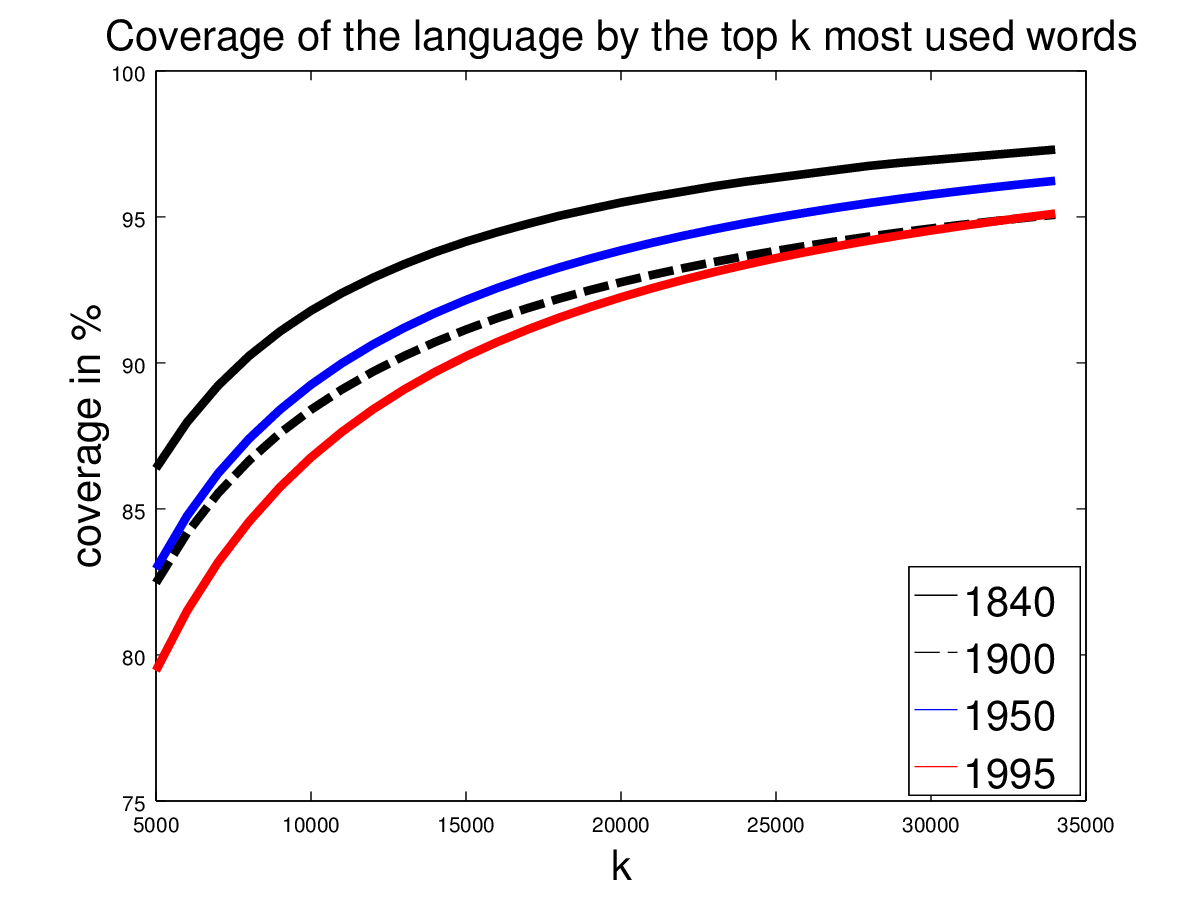
\includegraphics[scale=0.50]{Pictures/statistics/top-k-words-coverage/coverage.png}
    \caption{Percentage of text covered by the top k most used words}
    \label{coverage_figure}
\end{figure}

From those result, we can conclude that the number of new words grows faster with time passing than the number of disappearing words.
\subsection{Sentences and punctuation statistics}

We then did some statistics on the sentences and the punctuation. We started by analysing the average length of the sentences (see figure  \ref{average_sent_length_figure}).

\begin{figure}[H]
	\centering
    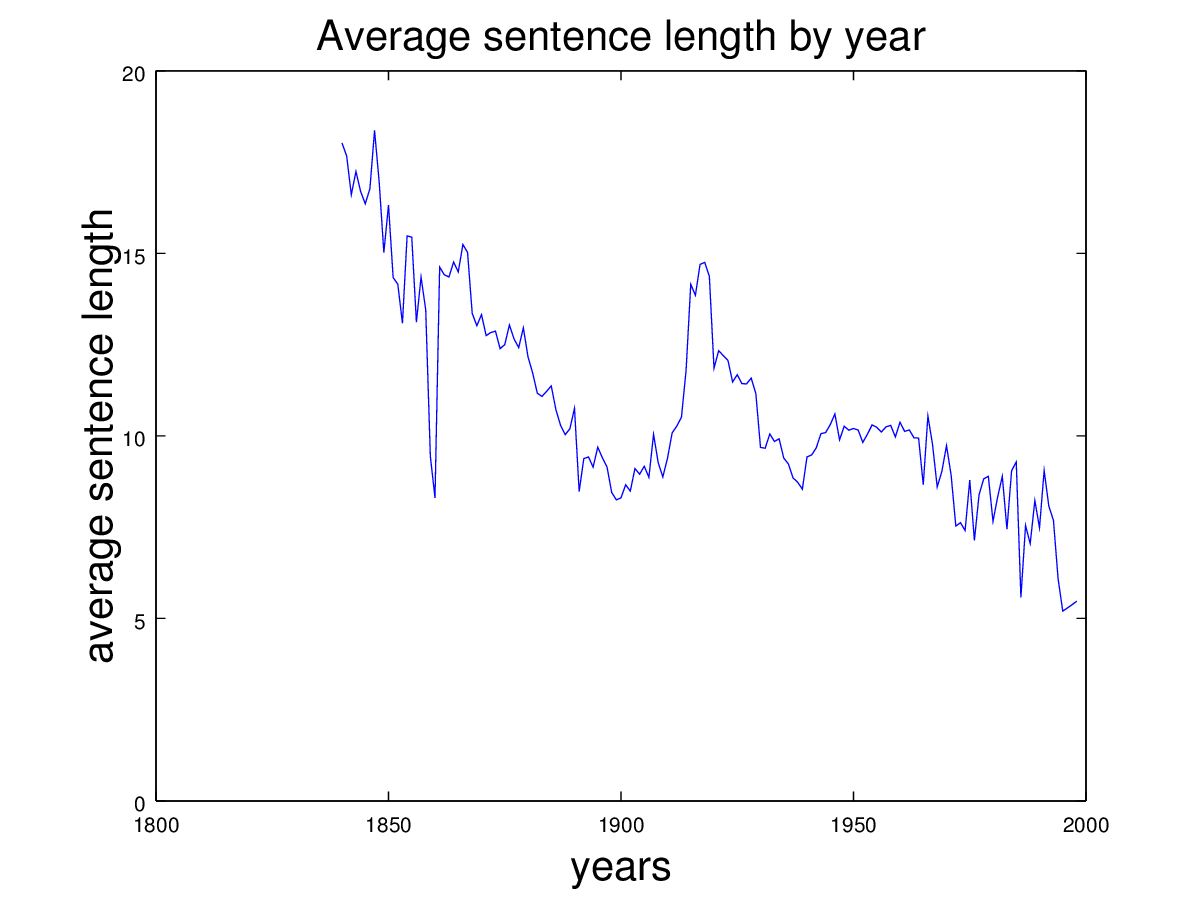
\includegraphics[scale=0.5]{Pictures/statistics/sentences-length/means.png}
    \caption{Average length of sentences by year}
    \label{average_sent_length_figure}\hfill
\end{figure}

\begin{figure}[H]
	\centering
    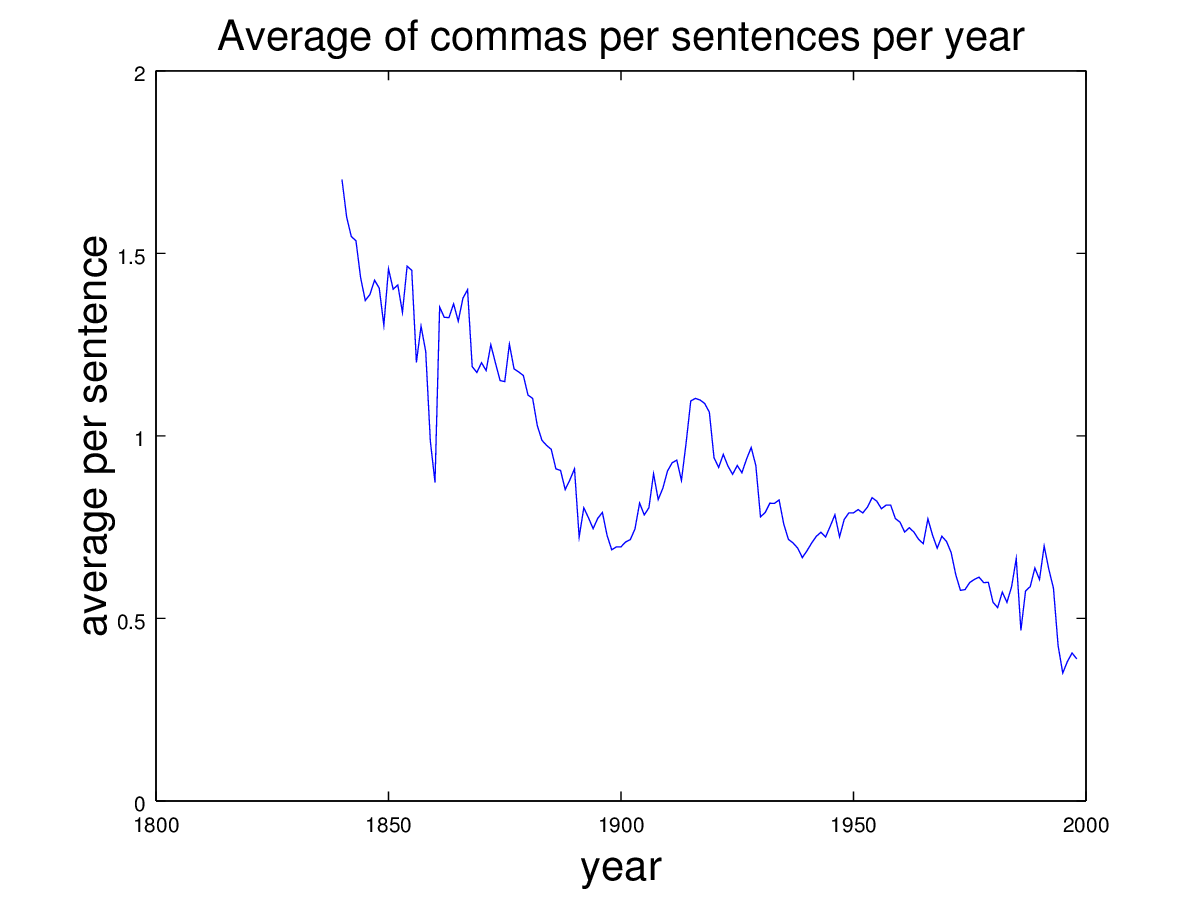
\includegraphics[scale=0.5]{Pictures/statistics/punctuation/graph.png}
    \caption{Average number of commas, semicolons and colons per sentence per year}
    \label{average_punct}\hfill
\end{figure}

If we ignore the down peak near 1850, coming from some unknown problem in two years (maybe less articles or big OCR problems) we see that the length of the sentences tends to decrease through time. In fact, the decrease is significant, going from 15-20 words by sentence in 1840 down to 8-10 words by sentence in 1990.

Note : another problem apart from the bad OCR is that from year 1917 to 1919 (included), we were provided with only one of the two newspapers merging into "Le Temps" articles, what affects the statistics for those years as there are less articles than in the other years.

We can correlate those results with the statistics on punctuation. In figure \ref{average_punct}, the black curve represents the average of commas per sentences per year, the red curve the average of semicolons and the blue curve the average of colons. The two last curves are not really interesting in terms of linguistic drift as they do not vary much. In fact, the articles are using approximatly the same number of colons and semicolons from 1840 to 1990. The black curve however show that, there is a tendency to use less commas on articles, what is quite logical as sentences are shorter so we need to use less commas.\\

Again, those statistics show the linguistic drift, between 1840 and 1990 by showing the fact that, through time, shorter sentences are used in our corpus. This trivially affects the punctuation used. \\

As those observations show a real variation between years, we thought it could be a good idea to use them for a metric. Results are presented in section \ref{dating}.

\subsection{Appearance of new words}

We consider the rate at which new 1-grams are incorporated in the vocabulary, and the nature of those words,  as a crucial component of linguistic drifts. It was thus important to come up with a reliable way to quantify this process .\\

A simple approach to estimate the apparition of new words would be to sum up the number of distinct 1-grams for each year and then monitor its evolution. But this suffers several drawbacks : first the remaining OCR errors, that still account for a substantial portion of the distinct 1-grams,  would be incorrectly considered as emerging words.  Furthermore, it would not provide any clue about the actual amount of words entering/exiting the set of used words, but only snapshots of how many words are in fashion at any point in time. Those two aspects would in our opinion have strongly distorted the resulting figures, this is why we opted for a different procedure.\\

The ideas was to define a pair of thresholds, one below which a word would be considered as not existing and a higher one meaning that the 1-gram is commonly used. The lower bound is not zero such as to take possible OCR correction into account. Once the higher threshold has been crossed, we require the frequencies to stay above the threshold R\% of the time.  This filter will only detect words that appear quite suddenly and as the advantage that we can determine the precise time where the words appeared (inferred from \textit{zerosSeqAtStart}). Figure \ref{algoschema} is meant to illustrate the algorithm.\\

\begin{figure}[h!]
        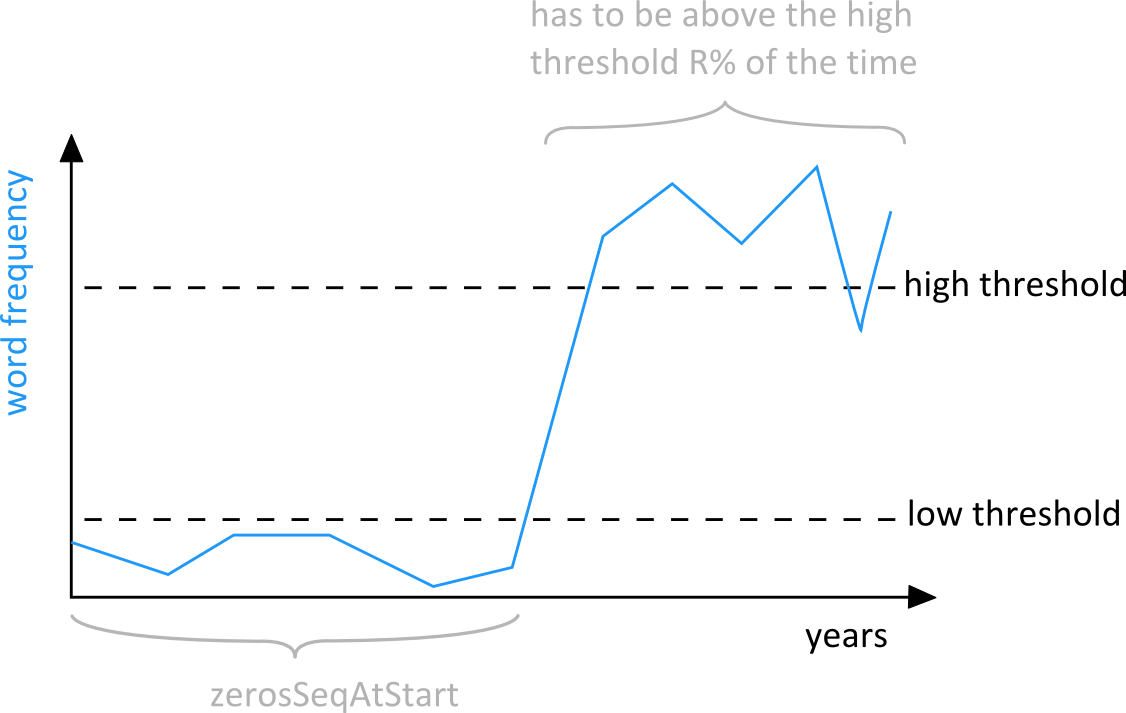
\includegraphics[scale=0.7]{Pictures/statistics/appearing-words/algo-schema.png}
        \caption{Visualization of the detection algorithm's behavior}
        \label{algoschema}
	\centering
\end{figure}

Figures \ref{ratio60} and \ref{ratio80} show the amounts of words spotted as appearing, using frequencies averaged over range of 5 years.  In our opinion the results for the first 15 year are overly influenced by the fact that they contains very few articles compared to other years (factor of 6). We see a clear increase in term of world creation recently, no matter the set of parameters selected. 
\begin{figure}[h!]
        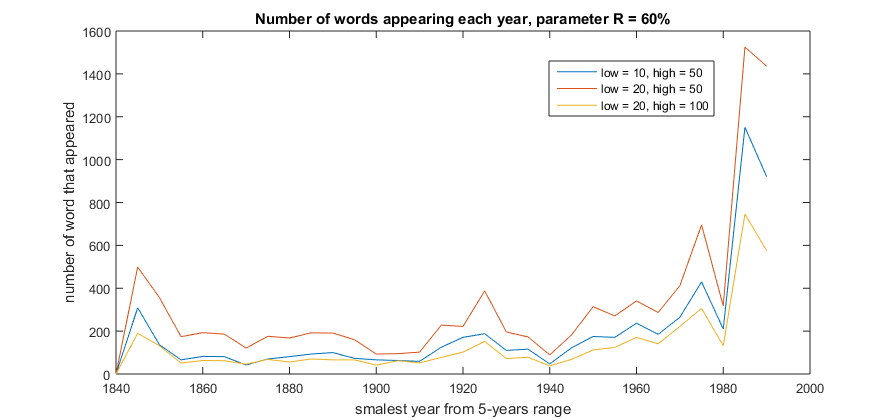
\includegraphics[scale=0.65]{Pictures/statistics/appearing-words/word-appearing-ratio60.png}
        \caption{New words detection with tolerance rate R = 60\%}
        \label{ratio60}
	\centering
\end{figure}
\begin{figure}[h!]
        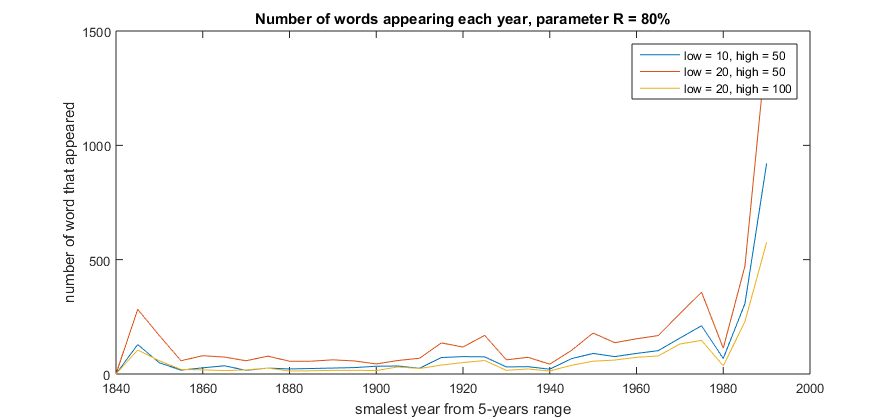
\includegraphics[scale=0.65]{Pictures/statistics/appearing-words/word-appearing-ratio80.png}
        \caption{New words detection with tolerance rate R = 80\%}
        \label{ratio80}
	\centering
\end{figure}
\subsection{Synonyms}

We have to remember that beyond n-grams frequency changes, there is also a shift in term of topics that are covered by newspapers over the years. To try to isolate our analysis from that effect, we planned to compare frequencies of words that have similar meaning using a synonym dictionary. After trying a few of them, we have chosen to use the myThes v2.0 synonym dictionary from OpenOffice that seemed exhaustive and accurate enough. \\

Frequency vectors were generated for every entry in the synonym database (using mapReduce) before being inserted in an SQL database. We have chosen to average frequencies to ranges of 5 years such as we limit the data size. Then we build a little web application that allows to check for words in the thesaurus database, then select a subset of the proposed similar words before displaying a plot with the evolution of frequencies.\\

This interactive application enabled us to quickly explore hypothesis we had about expected frequencies changes while, before, we needed to run a mapReduce job on the cluster for any chosen word. But most of the time, the synonyms proposed happen to have various meanings and were unsuitable to perform an automated analysis on our data. The intervention of the user was crucial during the selection phase to choose the appropriate ones. For instance a synonym for "voiture" (car) is "caisse" (slang) that also means box (by far its most frequent usage). Thus the perceived frequency of "caisse" will be strongly overstated and we cannot easily, at least for the scope of this project, tell apart the different meanings for a given 1-gram and split the occurrences accordingly.

\begin{figure}[H]
	\centering
        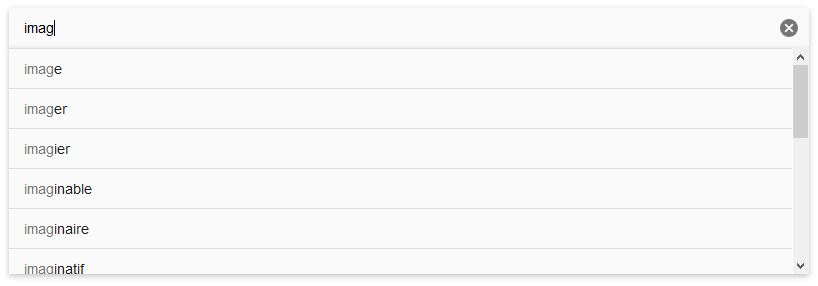
\includegraphics[scale=0.5]{Pictures/synonyms/search.jpeg}
        \caption{Seaching the thesaurus database with autocomplete}
        \label{search}
\end{figure}
\begin{figure}[H]
	\centering
        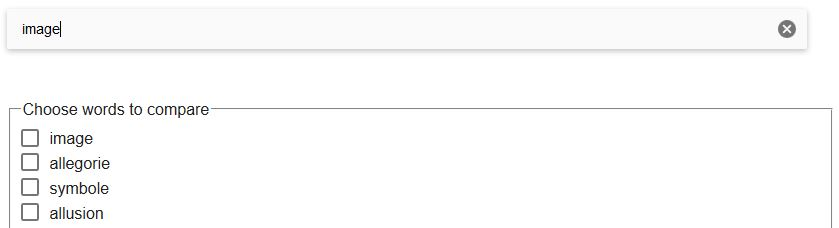
\includegraphics[scale=0.5]{Pictures/synonyms/select.jpeg}
        \caption{Check the proposed synonyms to display}
        \label{select}
\end{figure}

\begin{figure}[H]
	\centering
        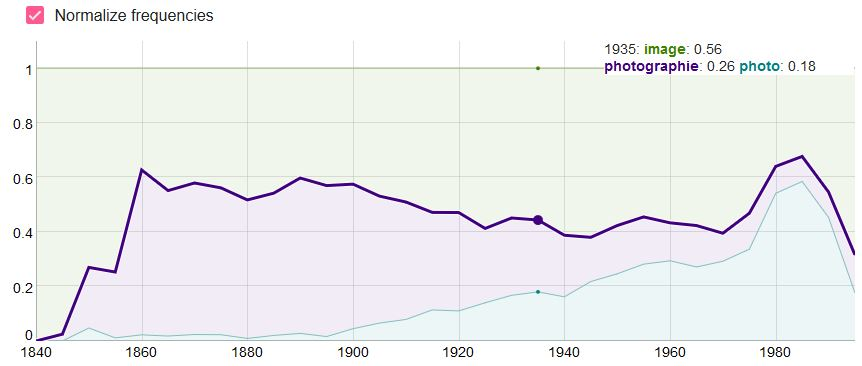
\includegraphics[scale=0.5]{Pictures/synonyms/graph.jpeg}
        \caption{Resulting frequency graph (with normalization option enabled)}
        \label{graph}
\end{figure}

\section{TF-IDF}

To try to accentuate the linguistic drift over the corpus, we thought it was a good idea to implement the \emph{Term Frequency} for each word in each year combined with the \emph{Inverse Document Frequency} which divides the number of documents in the corpus (years) by the number of documents where the word appears.

\begin{eqnarray}
    TF = \frac{\# \ of \ occurrences \ of \ a \ word \ in \ a \ year}{\# \ of \ words \ in \ a \ year}
\end{eqnarray}

\begin{eqnarray}
    IDF(t,D) = log \frac{N}{|\{d \in D : t \in d\}|}
\end{eqnarray}
where $N$ is the total number of documents (years) and $|\{d \in D : t \in d\}|$ is the number of documents where the word $t$ appears. We will see in the next sections of this paper that the TF-IDF values can be useful or not depending on the metric used.
\section{OCR Correction}
\subsection{Why do we need to clean the OCR?}

Limited by the optical character recognition, OCR documents comprise of a significant amount of erroneous words. Since our project rely heavily on word matching between documents, we need to deal with OCR error before we apply advance similarity calculation methods. 

Moreover, with all that said, the practical reality is that many OCR errors are quite predictable. So it is possible, and useful, to produce a pretty-good list of rules that simply translates individual tokens back into correctly spelled words. In this part, we utilized one simplest approach, i.e. to develop a set of rules to translate individual tokens produced by OCR errors back into correctly-spelled forms.

In order to found the impact of OCR correction, in the later section \ref{metrics} about metrics, we also experimented different metrics on OCR corrected dataset and OCR non-corrected dataset to find out whether OCR will play a significant effect upon the accuracy of metrics.

\subsection{Clean Strategy}
Since we need to pay more attention to the linguistic shift, here, for the OCR correction, we chose simplest approach and identified a set of predictable character substitutions. 

\begin{enumerate}[1.]
\item Basic Replacement Rule

We apply some common replacement rules to make the OCR word to be the same form.
	\begin{enumerate}[1.]
	\item Remove capital letter
	\item Remove alone letter
	\item Remove punctuation
	\item Remove accent
	\item Remove special letter (e.g., ;, /, -, ', \&)
	\end{enumerate}
\item Apply a set of predictable character substitutions

	In this part, we identified a set of common OCR error and do basic word replacement.

		\begin{enumerate}[1.]
		\item Replace complete word

		We replaced complete word if current n-grams exists a match with the word that in the dictionary, e.g., $so \rightarrow se$, $pir \rightarrow par$, $pavs \rightarrow pays$.

		\item Replace part of word

		For the matching of the partial word, we also use regular expression to find the corresponding word and its replacement word, e.g., $iii \rightarrow m$, $ii \rightarrow n$, $q.([a-z]) \rightarrow qu?$. Actually, most of wrong OCR words are local errors, and the substitution of local error plays a significant role in the OCR correction. 

		\end{enumerate}

\end{enumerate}

\section{Metrics}\label{metrics}
We look to determine a metric (or distance) between the years of the corpus that can show a linguistic drift. Intuitively, the language nowadays and 10 years ago is relatively the same, but there is more differences with the language 200 years ago. It a smooth evolution and we want to find a way to characterize it mathematically. Here are some intuitive properties for a distance $d$ between two subsets of the corpus $C_i$ and $C_{i'}$:

\begin{itemize}
 \item Normalization: $0 \leq d(C_i,C_{i'}) \leq 1$.
 \item Distance between a subset and itself is zero: $C_i = C_{i'} \Rightarrow d(C_i,C_{i'}) = 0$.
 \item The distance should be almost similar for consecutive years while increasing as years become distant.
 \item The distance should not depend on the size of the corpus.
\end{itemize}

In the following, distances will be represented in matrices of size $N \times N$, with $N = 159$ years is the interval of years building our corpus:
\[
\begin{matrix}
 & year1 & year2 & ... & yearN \\
 year1 & \mathbf{0} & \mathbf{d(year1,year2)} & ... & \mathbf{d(year1,yearN)} \\
 year2 & \mathbf{d(year2,year1)} & \mathbf{0} & ... & \mathbf{d(year2,yearN)} \\
 ... & ... & ... & ... \\
 yearN & \mathbf{d(yearN,year1)} & \mathbf{d(yearN,year2)} & ... & \mathbf{0}
\end{matrix}
\]
We tried several metrics that are presented in the next sections.

\subsection{Basic Distance}

In order to have a template and a point of comparison for our following work, we started with a simple and intuitive metric.

\subsubsection{The formula}

The distance calculation is based on the common words between two subsets $C_i$ and $C_{i'}$ of the corpus. The distance $d(C_i,C_{i'})$ is defined as follows:
\begin{eqnarray}
 d(C_i,C_{i'}) = 1 - \frac{2 \Arrowvert C_i \cap C_{i'}\Arrowvert}{\Arrowvert C_i \Arrowvert + \Arrowvert C_{i'} \Arrowvert }
\end{eqnarray}
where $\Arrowvert \cdot \Arrowvert$ denotes here the number of distinct words and $C_i \cap C_{i'}$ is the set containing the common words between $C_i$ and $C_{i'}$.

\subsubsection{Computations on the corpus}

We applied the basic distance on the years contained in the corrected corpus, producing the following matrix:

\begin{figure}[H]
    \centering
    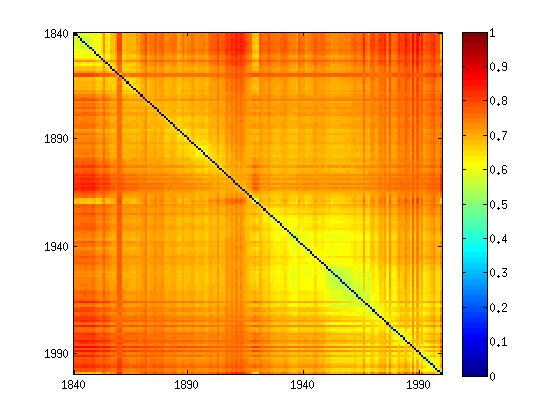
\includegraphics[scale=0.4]{Pictures/distance1/d1.jpg}
    \caption{Basic distance for 1-gram with OCR correction}
    \label{D1}
\end{figure}

\subsubsection{Analysis}

As our goal is to find a metric that can show a linguistic drift, consecutive years should have a distance near zero and distant years should have a distance close to one. In figure \ref{D1}, if we take for example the year 1940, the distance with itself is zero as wanted. But the distance with 1939 or 1941 is jumping over 0.5. Those kind of jumps around the zero diagonal are the behaviour we want to avoid and this distance is definitely not good.
\subsection{Chi-Square Distance}

The chi-square distance is often used in textual data analysis to find similarities between documents. It is very close to the euclidean distance (sum of squared differences between the elements) weighted by a term associated to the frequency of each word in the whole corpus.

\subsubsection{The formula}

In each subset $C_i$ of the corpus, we can denote $f_{i,j}$ the frequency of the word $w_j$. The distance is computed as follows:
\begin{eqnarray}
 d(C_i,C_{i'}) = \sum_j \frac{1}{f_{.j}} (\frac{f_{i,j}}{f_{i.}} - \frac{f_{i',j}}{f_{i'.}})^2
\end{eqnarray}
where $f_{i.} = \sum_j f_{i,j}$ is the total number of words contained in $C_i$ and $f_{.j} = \sum_i f_{i,j}$ is the frequency of the word $w_j$ over the entire corpus.

The term $f_{i,j}$ can also be replaced by the TF-IDF term.

\subsubsection{Computations on the corpus}

We applied the chi-square distance on the years contained in the corrected corpus, producing the following matrix:

\begin{figure}[H]
    \begin{minipage}[b]{0.48\linewidth}
        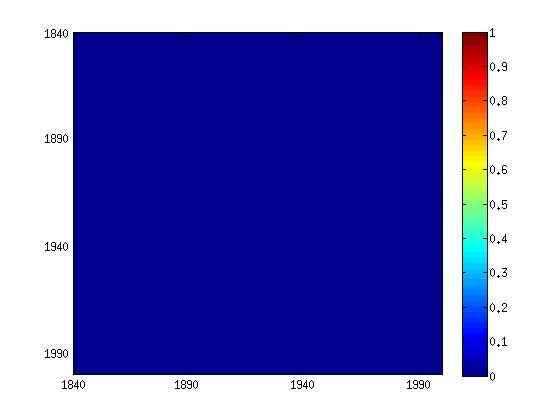
\includegraphics[scale=0.3]{Pictures/chi2/chi2_corrected2.jpg}
        \caption{chi-square distance for 1-gram with OCR correction}
        \label{chi2_1}
    \end{minipage}\hfill
    \begin{minipage}[b]{0.5\linewidth}
        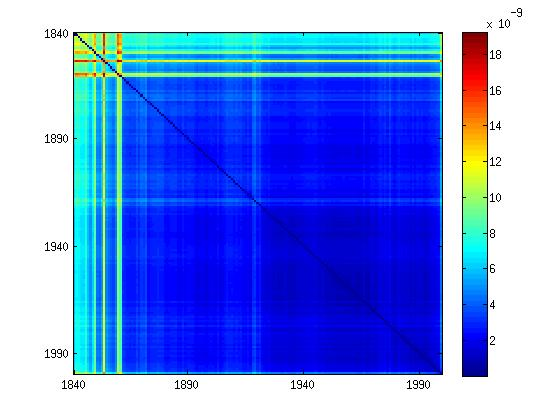
\includegraphics[scale=0.3]{Pictures/chi2/chi2_corrected.jpg}
        \caption{chi-square distance with reduced scale}
        \label{chi2_2}
    \end{minipage}\hfill
\end{figure}
\begin{figure}[H]
    \begin{minipage}[b]{0.48\linewidth}
        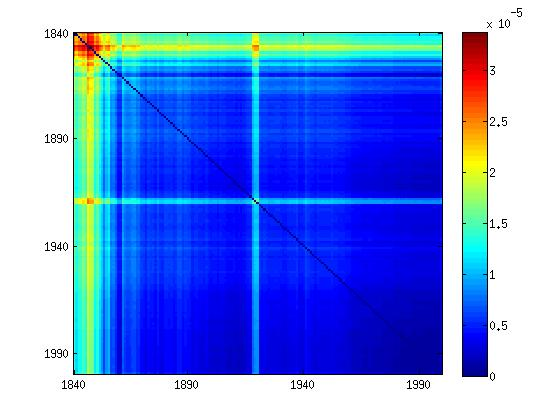
\includegraphics[scale=0.3]{Pictures/chi2/chi2_corrected_tfidf.jpg}
        \caption{chi-square distance weighted by TF-IDF}
        \label{chi2_tfidf}
    \end{minipage}\hfill
\end{figure}

\subsubsection{Analysis}

As we have a huge amount of articles for each year and that chi-square is used to compare documents, the maximal distance achieved is very low as shown in figure \ref{chi2_1}. In order to observe something we reduced the scale of the colours in figure \ref{chi2_2}. This distance is definitively smoother than the basic one but it doesn't show any evolution through the years.

Figure \ref{chi2_tfidf} shows the results when the terms of the distance are weighted by the TF-IDF coefficients. The values look similar than without the weighting.
\subsection{Cosine Similarity}

The cosine similarity is a measure between two vectors that is often used in documents research. It computes the cosine of the angle between both term vectors of the documents.

\subsubsection{The formula}

As the measure computes the similarity between two documents,  we will use $d(C_i,C_{i'}) = 1 - cosine\_ similarity$ to have a distance. In each subset $C_i$ of the corpus, we can denote $f_{i,j}$ the frequency of the word $w_j$. It is computed as follows:
\begin{eqnarray}
 d(C_i,C_{i'}) = 1 - \frac{\sum_j f_{i,j}\cdot f_{i',j}}{\sqrt{\sum_j f_{i,j}^2} \sqrt{\sum_j f_{i',j}^2 }}
\end{eqnarray}

The term $f_{i,j}$ can also be replaced by the TF-IDF term.

\subsubsection{Computations on the corpus}

We applied the cosine distance on the years contained in the corpus, producing the following matrices:

\begin{figure}[H]
    \begin{minipage}[b]{0.48\linewidth}
        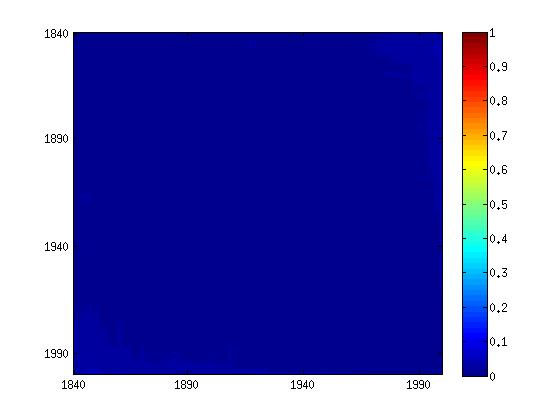
\includegraphics[scale=0.3]{Pictures/cos/cos_corrected2.jpg}
        \caption{cosine distance for 1-gram with OCR correction}
        \label{cos_1}
    \end{minipage}\hfill
    \begin{minipage}[b]{0.5\linewidth}
        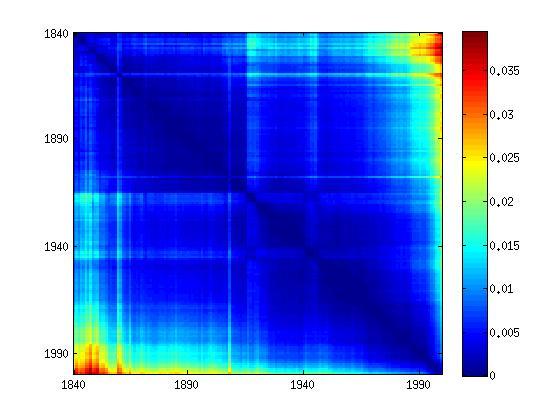
\includegraphics[scale=0.3]{Pictures/cos/cos_corrected.jpg}
        \caption{cosine distance with reduced scale on corrected corpus}
        \label{cos_2}
    \end{minipage}\hfill
\end{figure}
\begin{figure}[H]
    \begin{minipage}[b]{0.48\linewidth}
        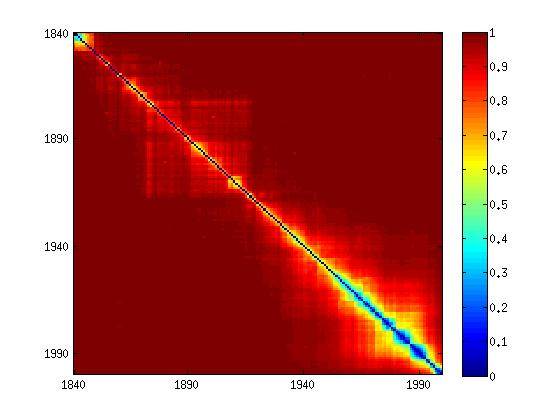
\includegraphics[scale=0.3]{Pictures/cos/cos_corrected_tfidf.jpg}
        \caption{cosine distance weighted by TF-IDF}
        \label{cos_tfidf}
    \end{minipage}\hfill
    \begin{minipage}[b]{0.48\linewidth}
        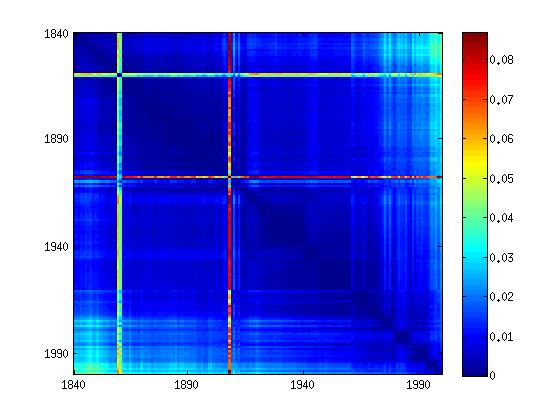
\includegraphics[scale=0.3]{Pictures/cos/cos_wo_corr.jpg}
        \caption{cosine distance on the corpus without correction}
        \label{cos_wo_corr}
    \end{minipage}\hfill
\end{figure}

\subsubsection{Analysis}

In the same manner as with the \emph{Chi-Square} distance, this measure is usually used to compare documents and not a huge set of articles containing a lot of common words. But in the rescaled matrix in figure \ref{cos_2}, we begin to have a more suited behaviour for our purpose. Indeed, it is smooth in the way that consecutive years have almost the same colour while there is a kind of band around the diagonal and a higher distance in the upper right and top left corners.

With the TF-IDF terms in figure \ref{cos_tfidf}, it is like if the values where all brought closer to the diagonal. We can see that 10 consecutive years look similar with each other and that the years after are much farther. It is not as smooth as expected for a good distance but it can be very useful and precise for dating.

In figure \ref{cos_wo_corr}, we can see the result of the cosine distance applied on the original OCR, without any correction. The red and yellow lines suggest that the OCR correction is useful and well done. It shows also that some particular years are affected a lot by OCR oddities.
\subsection{Kullback Leibler Divergence}

\subsubsection{The formula}
The \emph{Kullback-Leibler} (KL) Divergence does not mesure of the distance between subsets of the corpus, but the divergence between them. Indeed, let us consider sets $P$ and $Q$ containing articles for one year each. The KL divergence is defined as follows :

\begin{eqnarray}\label{KL}
    D_{KL}(P||Q) = \sum_i P(i) ln \frac{P(i)}{Q(i)}
\end{eqnarray}

It computes the sum of multiplications between the probability of the word $i$ in corpus $P$ and the natural logarithm of the same probability over the probability of the word $i$ in $Q$. Thus, $P$ and $Q$ need to be vectors containing the same words at the same indexes. We can also explain the \emph{Kullback-Leibler} Divergence as the loss of information
when $Q$ is used to approximate $P$ or, in other words, as the fact that $Q$ tries to simulate $P$.

Obviously, this divergence is not symmetric. Indeed, let us take for example two years $y_1$ and $y_2$ from the corpus. Suppose now that $y_1$ contains less distinct words than $y_2$. We can conclude that $y_2$ will have a better approximation of $y_1$ than the other way around, because $y_2$ has a bigger subset of words of $y_1$, so it can simulate it easily. We can observe this phenomenon in the following plots. The years around 1840 have some difficulties to simulate 1990's years but in the other direction it is easy because there is more vocabulary in the 20th century than in the 19th.\\

To compute this formula, as we need to have vectors with the same size representing the same words in the same order but some words appear only in certain years, we need to add the missing words in each year with a number of occurrences equal to 0. Doing so, we have for each year a vector containing all words over the whole corpus. With KL Divergence, we have to be careful, because if $P(i)$ or $Q(i)$ is 0, the computation will be totally wrong. Thus, we have to add some smoothing in the KL computation. We made the choice to add a really small value ($10^{25}$) and to weight it with the probability of the word over the whole corpus. Thus, we keep a small difference between words that appear a lot in the corpus and the ones that are less frequent\footnote{It is a way to take less into account for words that appear not that much, like words that does not exist in french and that we were not be able to correct perfectly.}.

\subsubsection{Computations on the corpus}
We computed the \emph{Kullback-Leibler} Divergence with the non-corrected corpus and the OCR-corrected corpus. We also used the probability that a word appears in a year and the TF-IDF value of each one. The explanations about the plots are located below.

\begin{figure}[H]
    \begin{minipage}[b]{0.48\linewidth}
        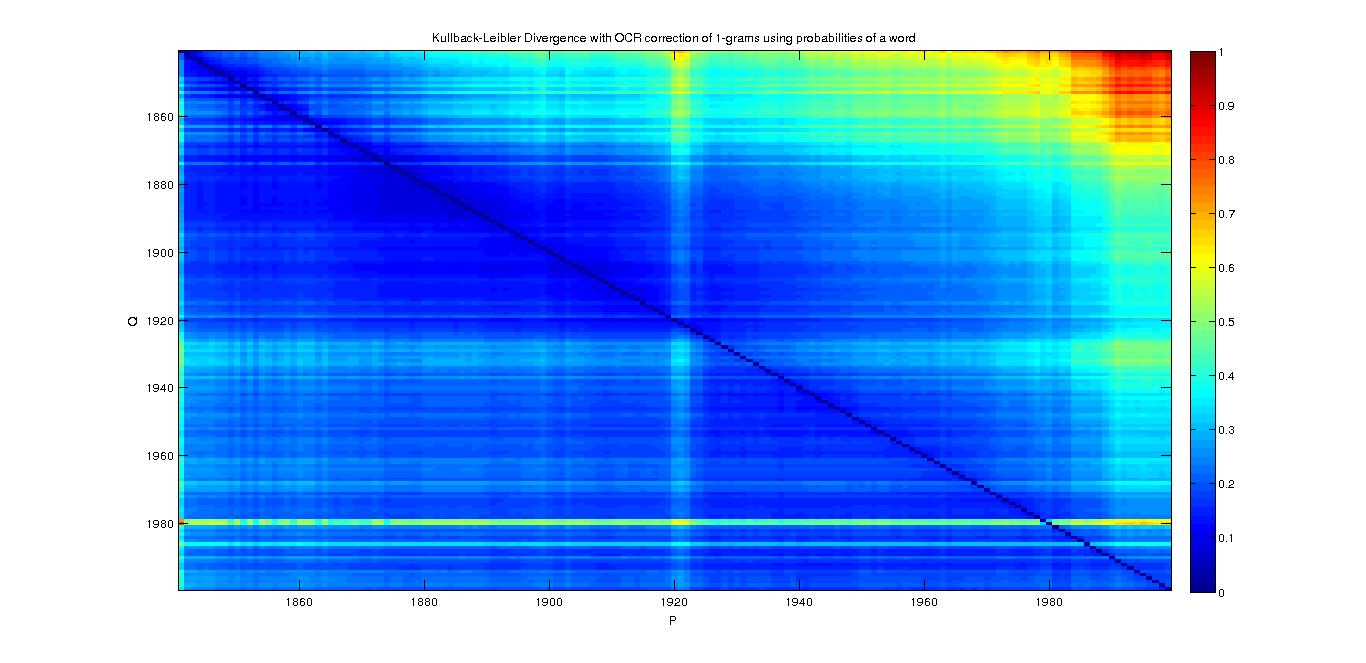
\includegraphics[scale=0.25]{Pictures/kullback-leibler/KL_1-grams_with_correction_proba.jpg}
        \caption{KL for 1-gram with OCR correction and probability of word}
        \label{KL-PC1}
    \end{minipage}\hfill
    \begin{minipage}[b]{0.5\linewidth}
        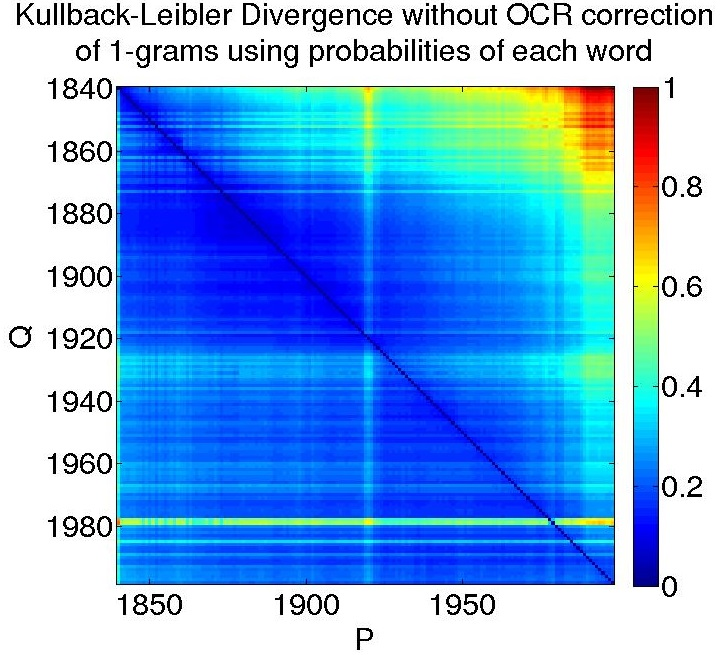
\includegraphics[scale=0.25]{Pictures/kullback-leibler/KL_1-grams_without_correction_proba.jpg}
        \caption{KL for 1-gram without OCR correction and probability of word}
        \label{KL-PN1}
    \end{minipage}\hfill
\end{figure}

\begin{figure}[H]
    \begin{minipage}[b]{0.48\linewidth}
        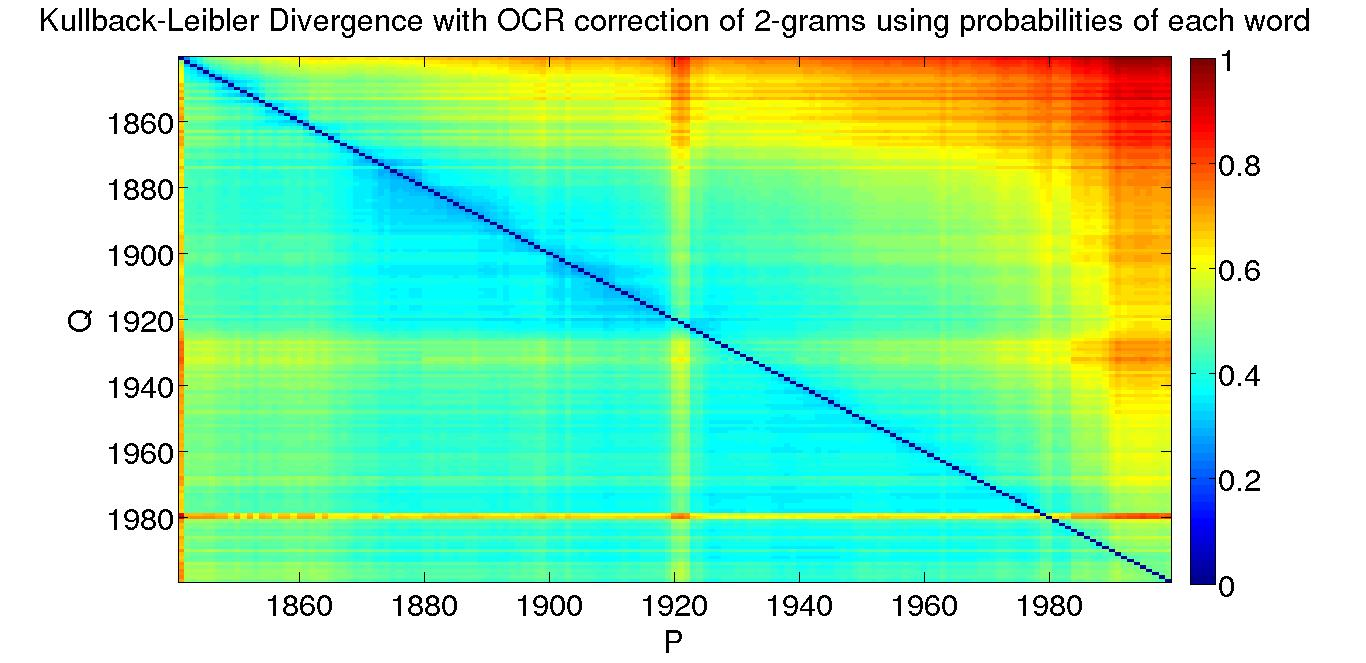
\includegraphics[scale=0.25]{Pictures/kullback-leibler/KL_2-grams_with_correction_proba.jpg}
        \caption{KL for 2-grams with OCR correction and probability of word}
        \label{KL-PC2}
    \end{minipage}\hfill
    \begin{minipage}[b]{0.5\linewidth}
        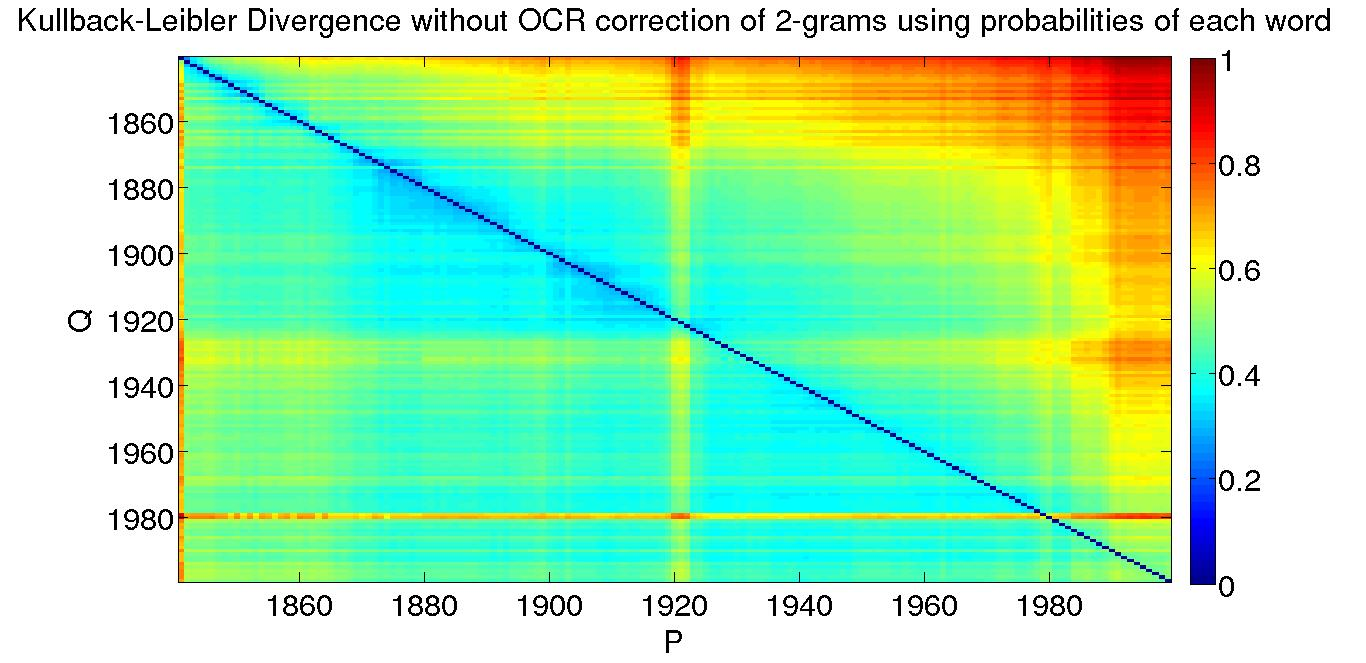
\includegraphics[scale=0.25]{Pictures/kullback-leibler/KL_2-grams_without_correction_proba.jpg}
        \caption{KL for 2-grams without OCR correction and probability of word}
        \label{KL-PN2}
    \end{minipage}\hfill
\end{figure}

\begin{figure}[H]
    \begin{minipage}[b]{0.48\linewidth}
        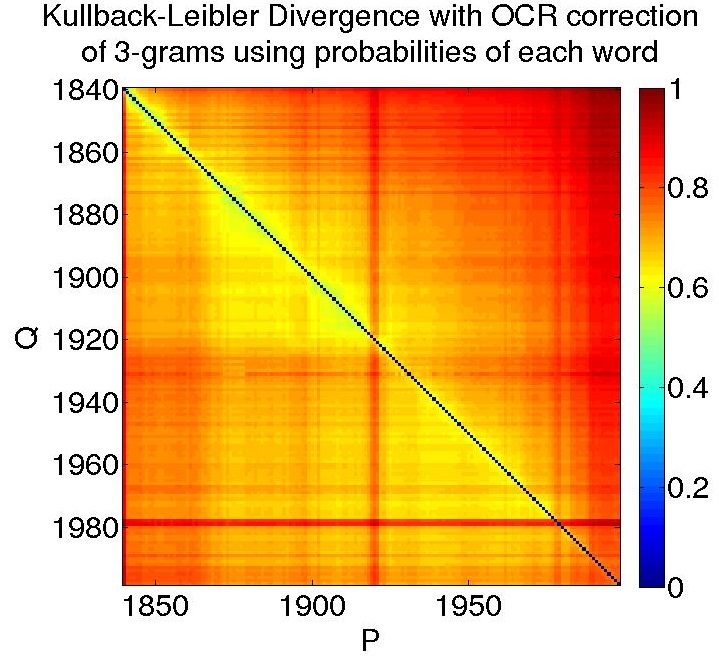
\includegraphics[scale=0.25]{Pictures/kullback-leibler/KL_3-grams_with_correction_proba.jpg}
        \caption{KL for 3-grams with OCR correction and probability of word}
        \label{KL-PC3}
    \end{minipage}\hfill
    \begin{minipage}[b]{0.5\linewidth}
        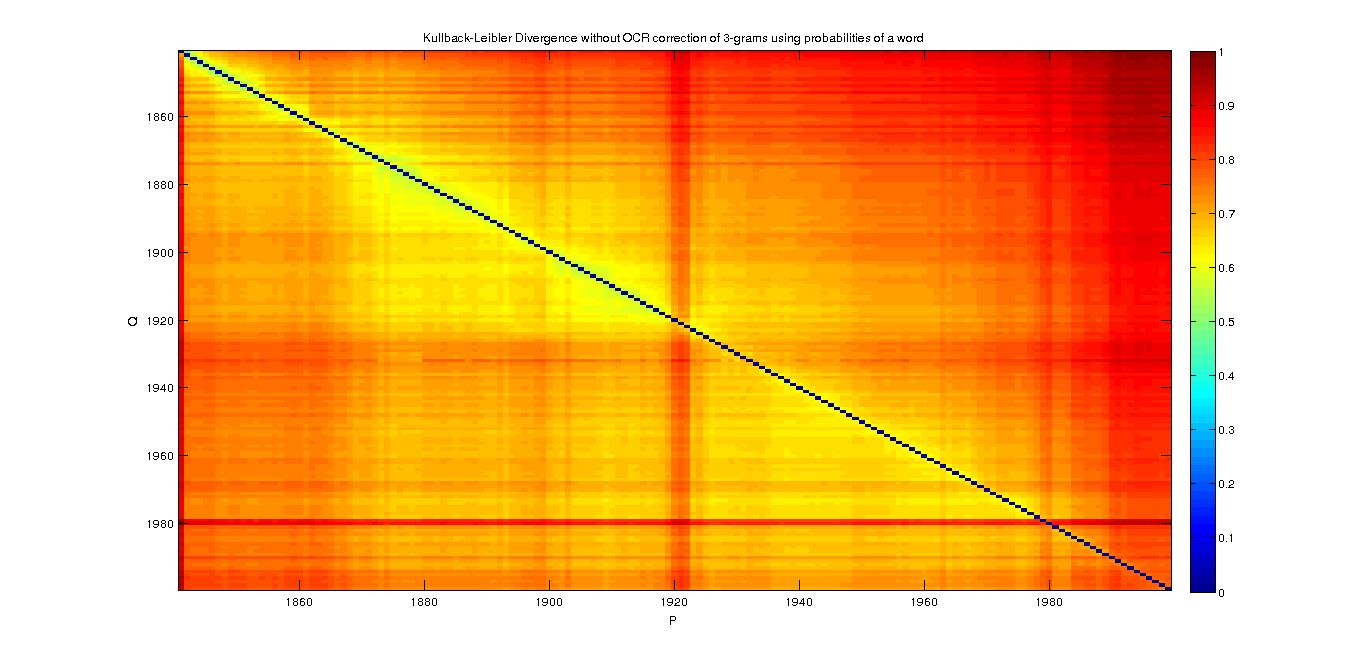
\includegraphics[scale=0.25]{Pictures/kullback-leibler/KL_3-grams_without_correction_proba.jpg}
        \caption{KL for 3-grams without OCR correction and probability of word}
        \label{KL-PN3}
    \end{minipage}\hfill
\end{figure}

\begin{figure}[H]
    \begin{minipage}[b]{0.48\linewidth}
        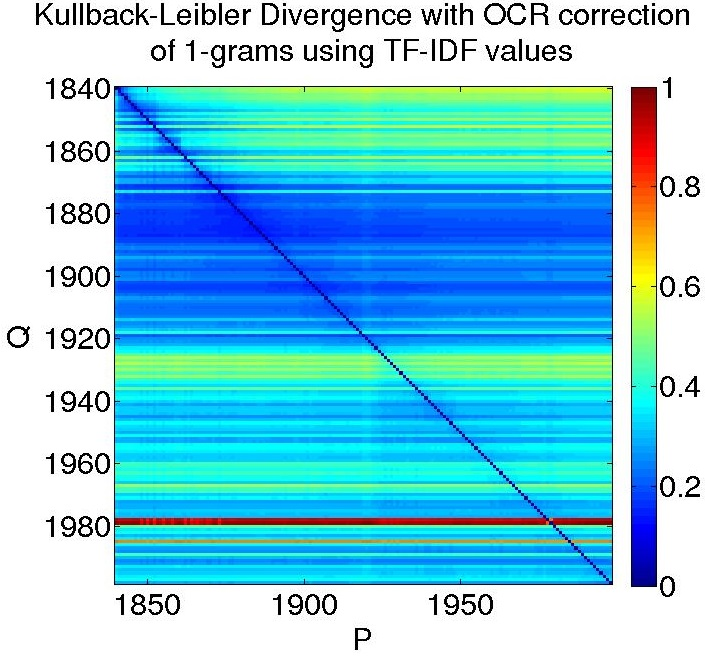
\includegraphics[scale=0.25]{Pictures/kullback-leibler/KL_1-grams_with_correction_tfidf.jpg}
        \caption{KL for 1-gram with OCR correction and TF-IDF}
        \label{KL-TC1}
    \end{minipage}\hfill
    \begin{minipage}[b]{0.5\linewidth}
        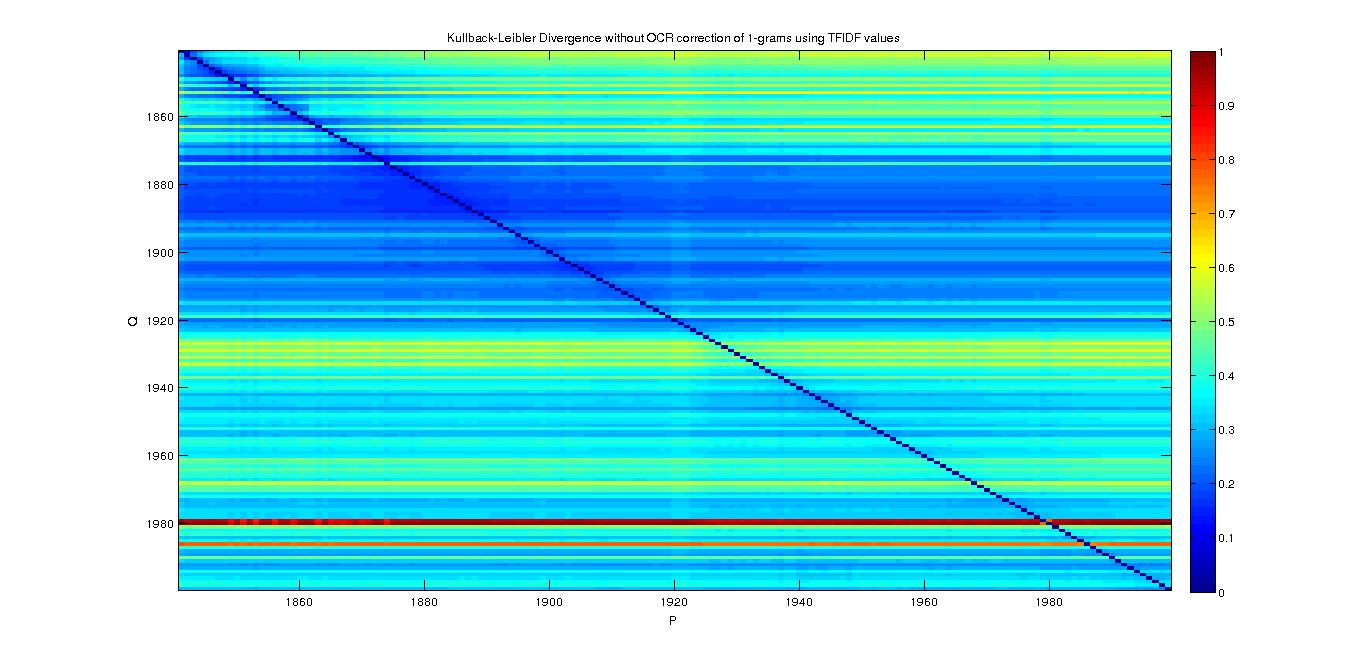
\includegraphics[scale=0.25]{Pictures/kullback-leibler/KL_1-grams_without_correction_tfidf.jpg}
        \caption{KL for 1-gram without OCR correction and TF-IDF}
        \label{KL-TN1}
    \end{minipage}\hfill
\end{figure}

\begin{figure}[H]
    \begin{minipage}[b]{0.48\linewidth}
        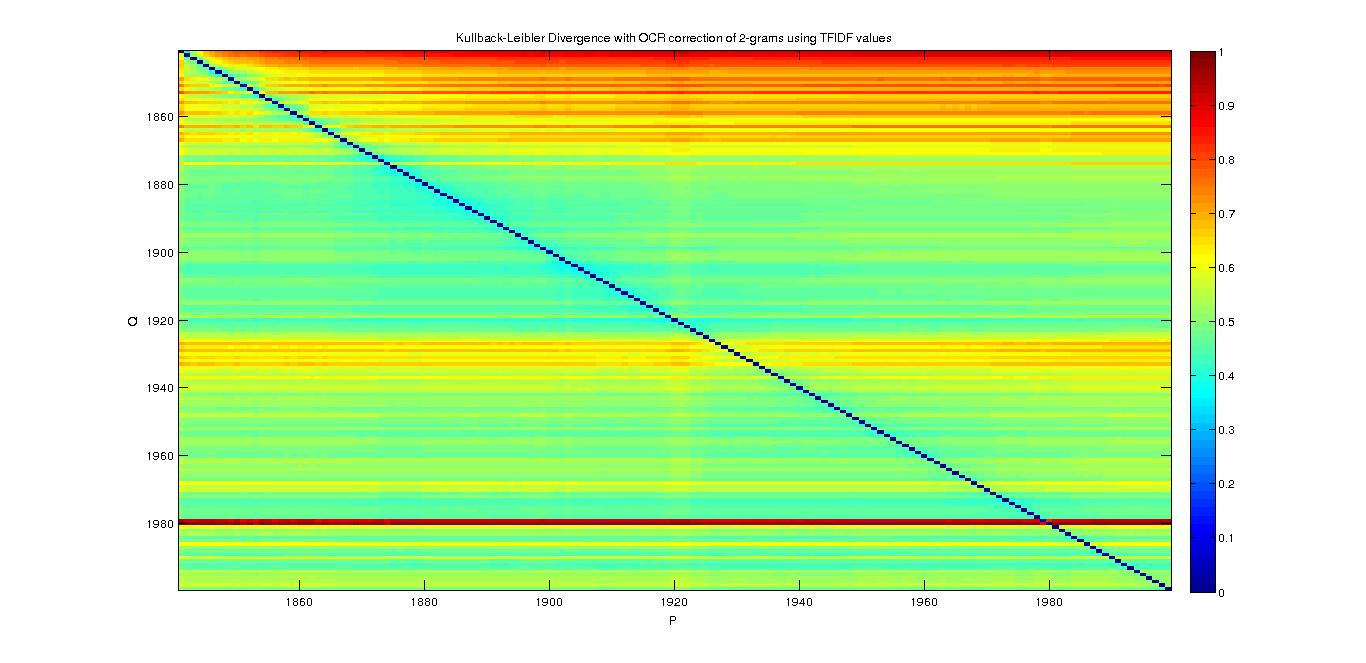
\includegraphics[scale=0.25]{Pictures/kullback-leibler/KL_2-grams_with_correction_tfidf.jpg}
        \caption{KL for 2-grams with OCR correction and TF-IDF}
        \label{KL-TC2}
    \end{minipage}\hfill
    \begin{minipage}[b]{0.5\linewidth}
        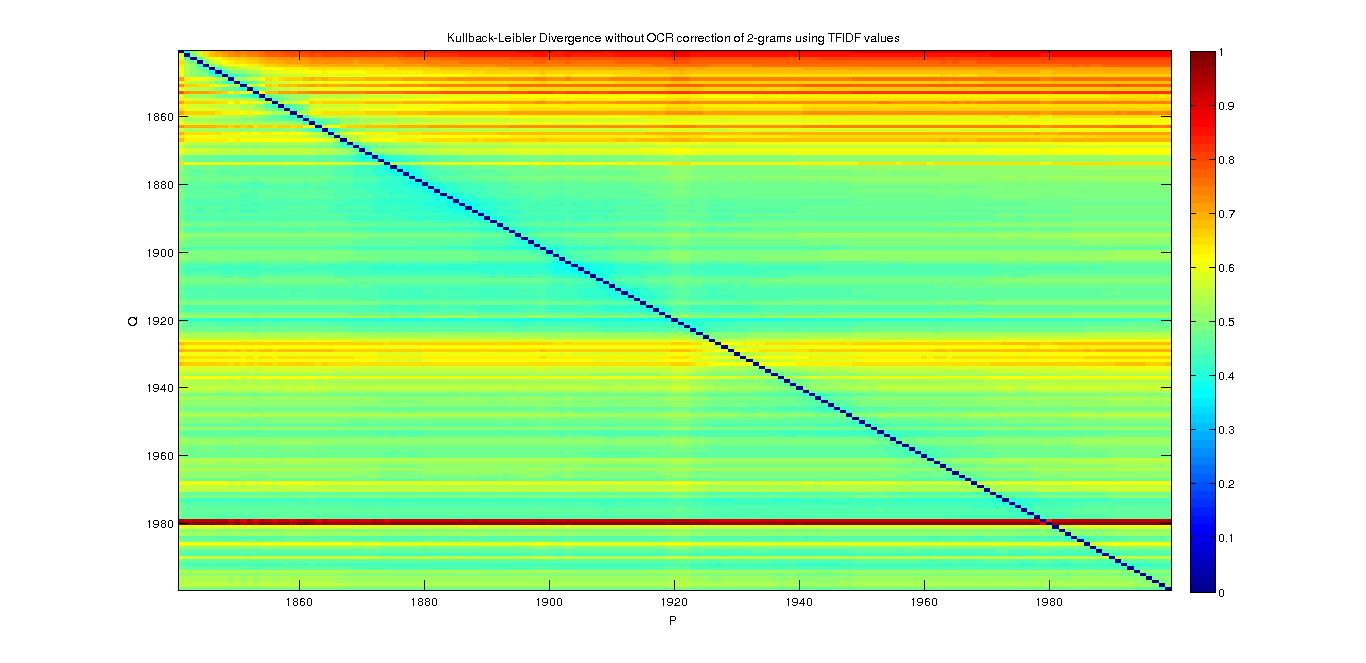
\includegraphics[scale=0.25]{Pictures/kullback-leibler/KL_2-grams_without_correction_tfidf.jpg}
        \caption{KL for 2-grams without OCR correction and TF-IDF}
        \label{KL-TN2}
    \end{minipage}\hfill
\end{figure}

\begin{figure}[H]
    \begin{minipage}[b]{0.48\linewidth}
        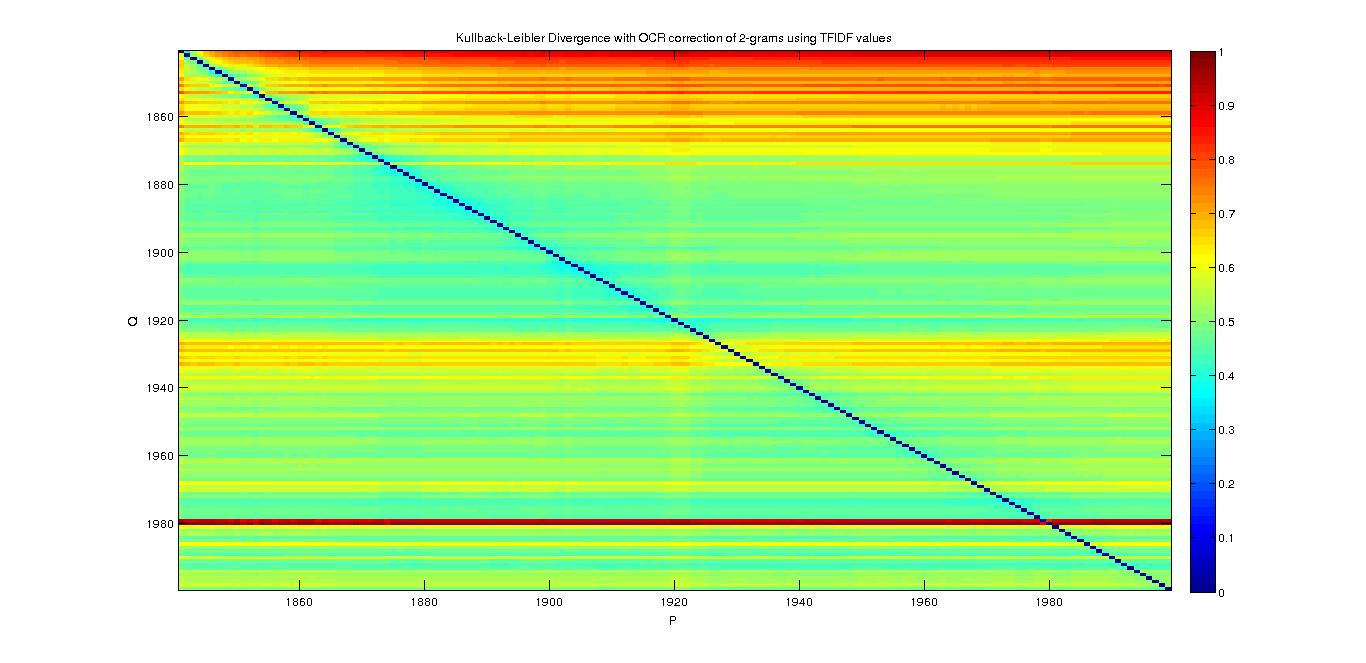
\includegraphics[scale=0.25]{Pictures/kullback-leibler/KL_2-grams_with_correction_tfidf.jpg}
        \caption{KL for 3-grams with OCR correction and TF-IDF}
        \label{KL-TC3}
    \end{minipage}\hfill
    \begin{minipage}[b]{0.5\linewidth}
        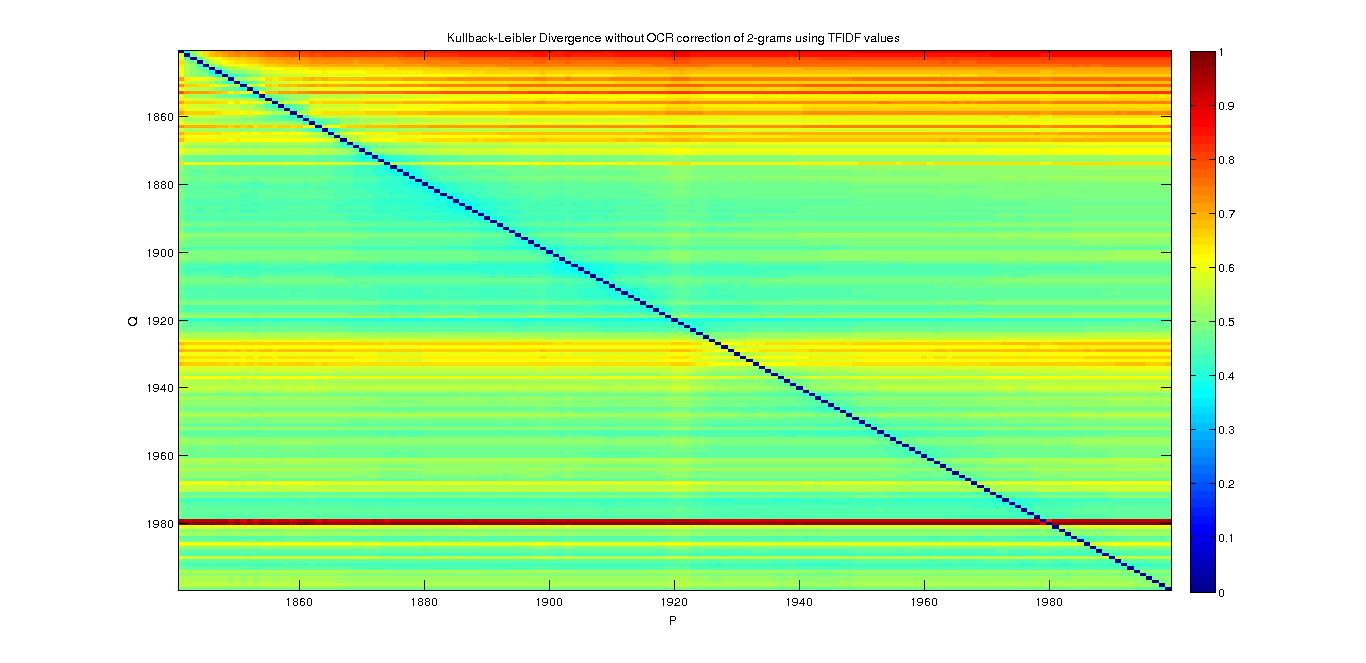
\includegraphics[scale=0.25]{Pictures/kullback-leibler/KL_2-grams_without_correction_tfidf.jpg}
        \caption{KL for 3-grams without OCR correction and TF-IDF}
        \label{KL-TN3}
    \end{minipage}\hfill
\end{figure}

\subsubsection{Analysis of results}
As we can observe, there is no real difference between the results of the metric applied to the non-corrected corpus and the results of the metric applied to the corrected one. Thus, we can assume that the OCR correction is not really helping to compute the distance between articles from each year. The interesting fact is that the upper right corner in each plot with the probability of a word (figures \ref{KL-PC1} to \ref{KL-PN3}) has a higher divergence value than the rest of the plot. It is, as explained in the section of this report about synonyms, due to the fact that words tend to increase in number of words rather than disappear. Indeed, if we have less words in 1840 and much more in 1998, it is obvious that when we approximate 1840 with 1998, the divergence is low and when we approximate 1998 with 1840 it is more difficult (right upper corner).

Augmenting the degree of n-grams, we can observe that, generally, the plots become more red because the divergence is bigger, which is totally understandable (we have n-grams that occur less, so it the approximation of a year with another one becomes more difficult). With the 2-grams, the "red part" is larger in the right upper corner and with the 3-grams, all the plot becomes red. In the 3-grams plot, we can also see that there is a light tight band around the diagonal, which indicates us that the articles from close years share a bigger set of words.

The results of \emph{Kullback-Leibler} divergence with TF-IDF (figures \ref{KL-TC1} to \ref{KL-TN3}) are really strange and have always the same form (for 1,2 and 3-grams). It is difficult to explain why it has this form, but a possible explanation could be that the TF-IDF gives more importance to the words that appears less in the corpus. Knowing that we try to approximate a year with another one, it is obvious that it becomes difficult to approximate a year if the uncommon words have more weight. It can explain the lines in the plots, because a year could have the same difficulties to approximate each other year.

\subsection{Out of Place Measurement}

\subsubsection{Metric description}

This measure determines how far out of place an n-gram in one profile is from its place in the other profile. It allows us to consider the change in the importance of common word of the two corpuses. The rank of the n-gram is its order by its frequency. If a word appears or disappear it has a maximum value rank. Otherwise, we sum to the metric the change of rank of the n-gram. The process of computation can be concluded as follows:

\begin{eqnarray}\label{outofplace}
	D(i, j) = \sum_{x \in D_i \bigcap x \in D_j} |R_x^i - R_x^j| + 
			\max_{x \in D_i \bigcap x \in D_j}(R_x^i - R_x^j) (\sum_{x \in (D_i - D_j)} 1 + \sum_{x \in (D_j - D_i)} 1)
\end{eqnarray}

\subsubsection{Computation of \emph{Out of Place} measurement}

In the experiment, the \emph{Out of Place} measurement is divided to two methods (i.e., whether to use the unmatched word's frequency. We also computed the \emph{Out of Place} with the non-corrected corpus and the OCR-corrected corpus to see the impact of OCR correction. The figures illustrated below explain the performance of \emph{Out of Place} under different conditions in the dataset of 1-gram. For the experiment on 2-gram and 3-gram, they have similar performance to 1-gram, and details are omitted.

\begin{figure}[H]
    \begin{minipage}[b]{0.48\linewidth}
        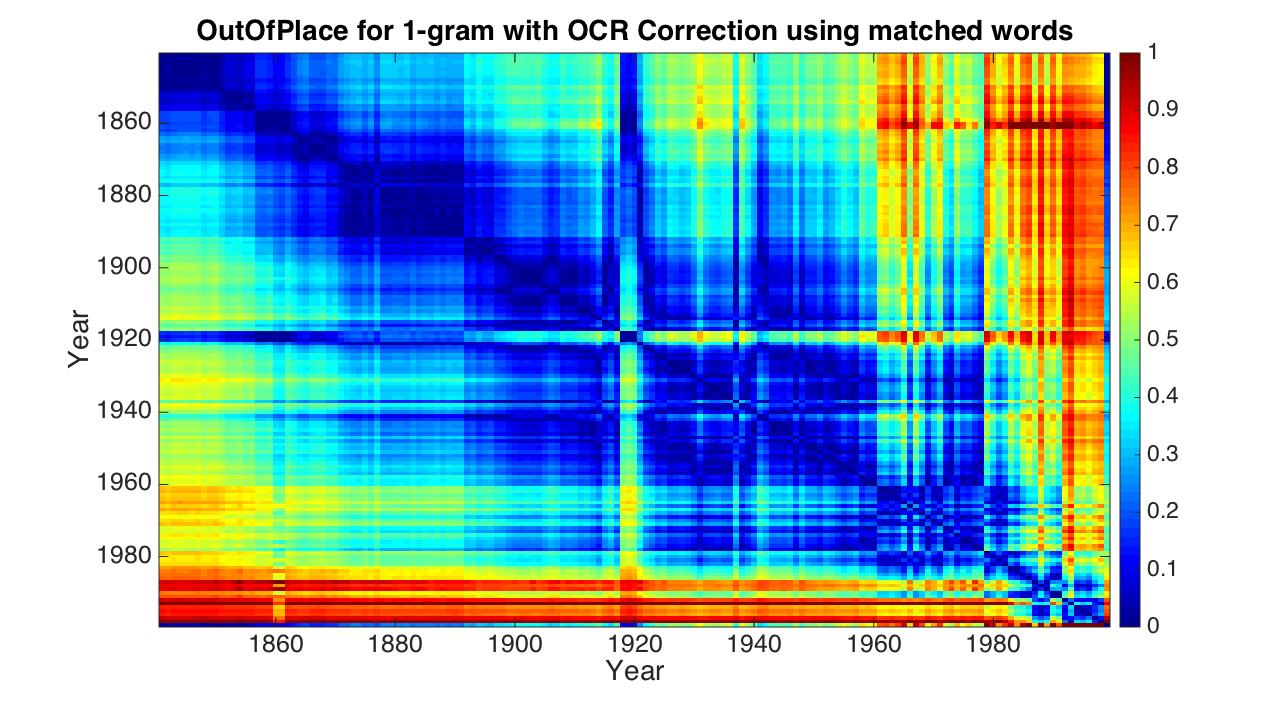
\includegraphics[scale=0.15]{Pictures/outofplace/outofplace_1-gram_correctedOCR_matched_words.jpg}
        \caption{Outofplace for 1-gram with OCR correction using matched words}
        \label{outofplace_1_match_correct}
    \end{minipage}\hfill
    \begin{minipage}[b]{0.5\linewidth}
        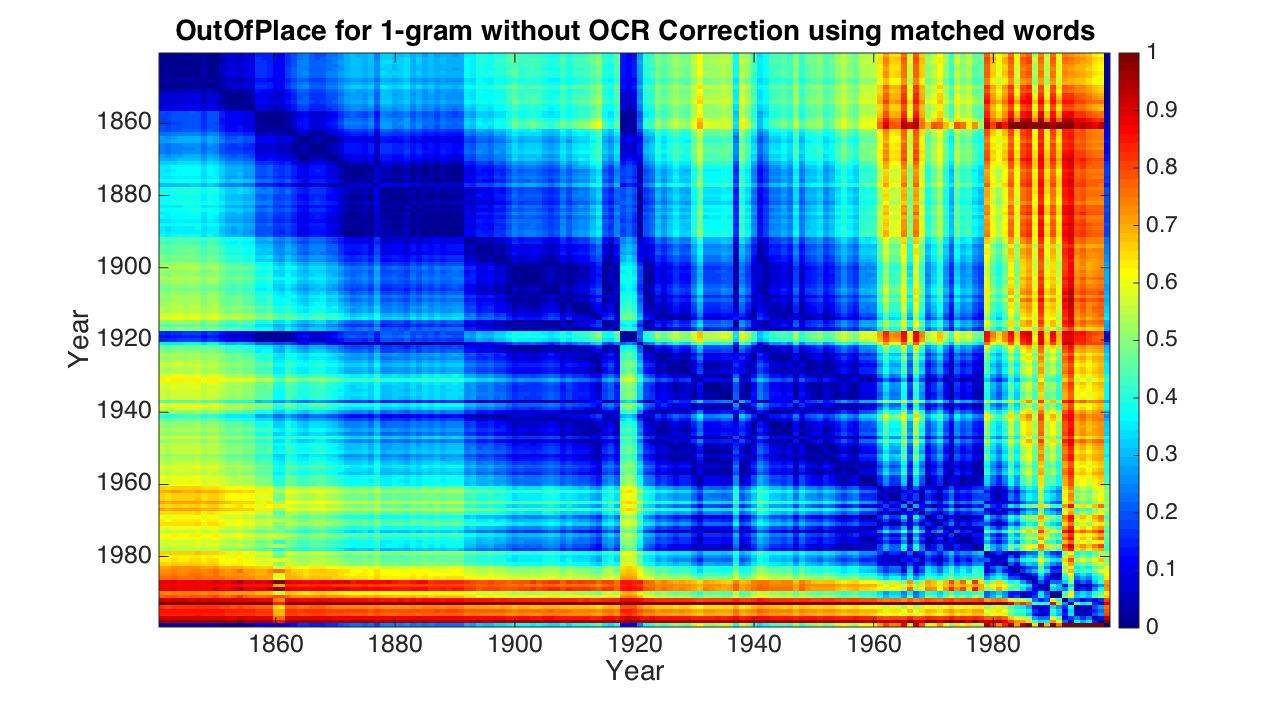
\includegraphics[scale=0.15]{Pictures/outofplace/outofplace_1-gram_noncorrectedOCR_matched_words.jpg}
        \caption{Outofplace for 1-gram without OCR correction using matched words}
        \label{outofplace_1_match_noncorrect}
    \end{minipage}\hfill
\end{figure}

\begin{figure}[H]
    \begin{minipage}[b]{0.48\linewidth}
        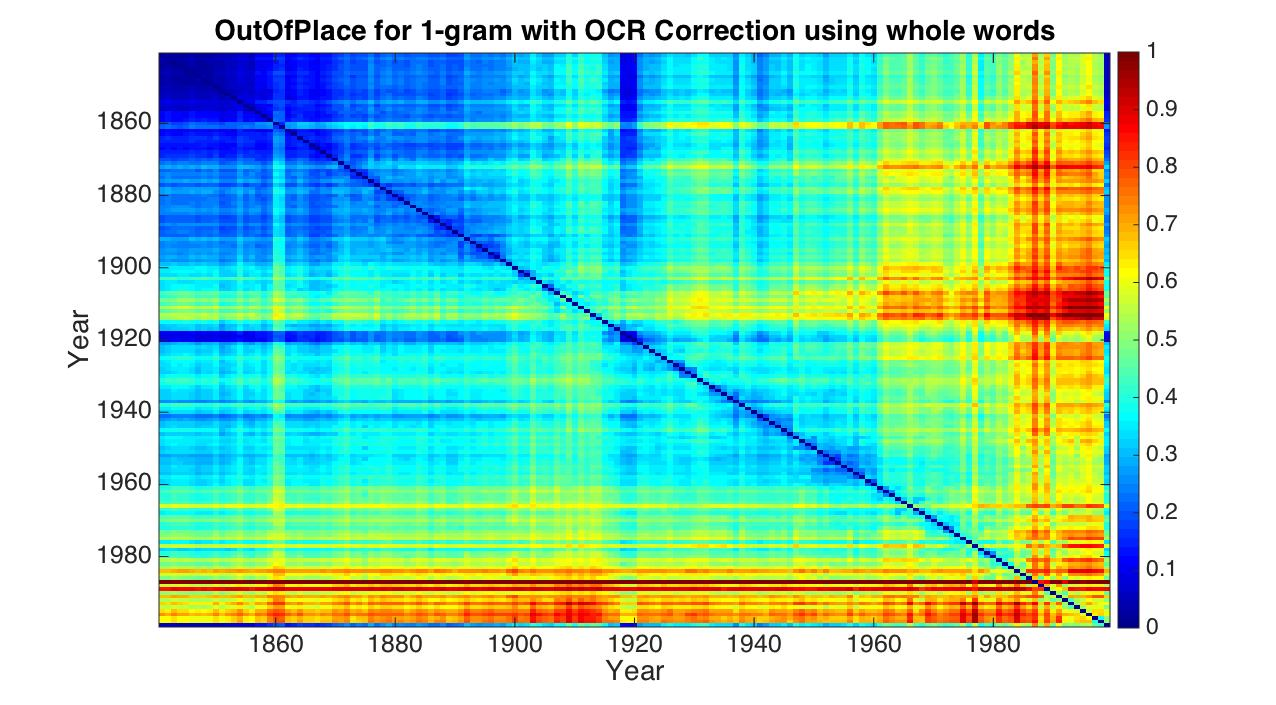
\includegraphics[scale=0.15]{Pictures/outofplace/outofplace_1-gram_correctedOCR_whole_words.jpg}
        \caption{Outofplace for 1-gram with OCR correction using whole words}
        \label{outofplace_1_all_correct}
    \end{minipage}\hfill
    \begin{minipage}[b]{0.5\linewidth}
        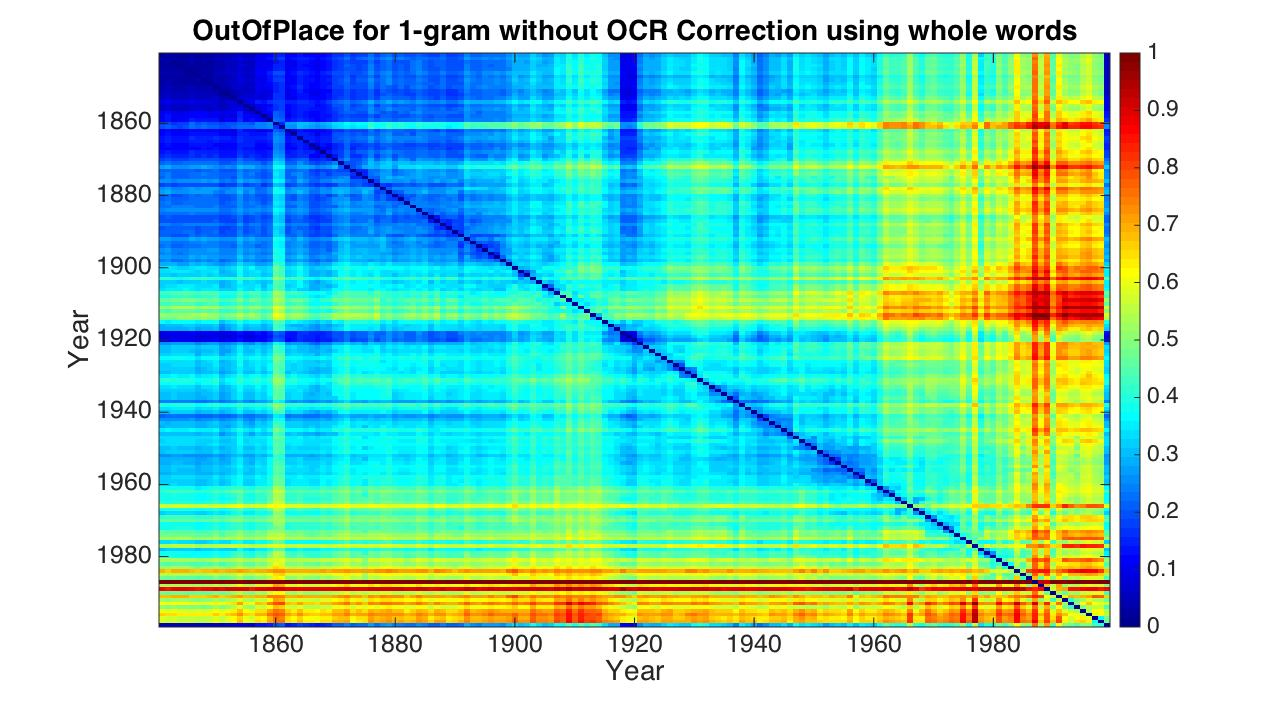
\includegraphics[scale=0.15]{Pictures/outofplace/outofplace_1-gram_noncorrectedOCR_whole_words.jpg}
        \caption{Outofplace for 1-gram without OCR correction using whole words}
        \label{outofplace_1_all_noncorrect}
    \end{minipage}\hfill
\end{figure}

\subsubsection{Analysis of results}

We can witness that for this method, the effect of OCR correction is not clear: For the same metric strategy but using different dataset (i.e., OCR corrected dataset and OCR non-corrected dataset), it has few changes in ratio but more in count (see figures \ref{outofplace_1_match_correct} and \ref{outofplace_1_match_noncorrect}; figures \ref{outofplace_1_all_correct} and \ref{outofplace_1_all_noncorrect}). More accurately, the increased count obtained by \emph{Out of Place} measurement does not affect the global picture, since most of data also increase by a similar ratio. But the feature shown by comparison is close to the description of original paper that \emph{Out of Place} provides high robustness in the face of OCR error.

However, the decision that whether we should use those unmatched words greatly impact the final distance between different years. If we only use matched words, then its result seems acceptable (see figures \ref{outofplace_1_match_correct}) where we can witness that the distance is small when comparable year is close to current year, and the distance normally increased followed by the distance between different years. But there also exists a strange phenomenon around the year $1920$ that the word appears in this year is close to the word in previous 40 to 80 years. Checking the performance of other metric in the year $1917$ to $1919$, we can also find a similar condition (e.g., Kullback Leibler Divergence, Chi-square) because one of the two newspapers is missing for those years.

When it comes to the result that utilized whole words including unmatched word (see \ref{outofplace_1_all_correct}), we can witness that before year $1960$, the metric shows a good performance that closes to the rule that it ought to be. However, after year $1960$, the distance between current year and comparable year is extremely high and badly decrease the quality of this metric. We will using these two approaches in the part of dating article to find out a proper approach to fit ours dataset.


\section{Dating Articles}\label{dating}
Having some metrics to compare the articles between years, we thought it was a good idea to try to date a subset of articles from a year with these metrics. Thus, we wrote a \emph{Scala} application that selects a subset of articles in a year and we considered this subset of articles as a year to be able to reuse the same code as for the comparison between years. Nevertheless, we had to adapt a bit our codes because it was unnecessary to compare years with years but only articles with years. We also had to remove the articles from the year they belong to. Finally, we selected a subset of articles and not only one article because in the corpus, some titles of articles in the newspaper are considered as a complete article. Thus, it has no sense to have the possibility to select only one article with 4 or 5 words.\\

You can find below the different results for the different metrics with the years 1880, 1920 and 1995 and with taking 15 articles in each year.

\subsection{Metrics}

\subsubsection{Basic Distance}
\subsubsection{Chi Square}
\subsubsection{Cosine}
\subsubsection{Cosine with TF-IDF}
\subsubsection{Kullback-Leibler Divergence}
Figures \ref{ArticleKL-C1880} to \ref{ArticleKL-N1995} show the results for the 3 different years trying to represent the articles with each year :

\begin{figure}[h!]
    \begin{minipage}[b]{0.48\linewidth}
        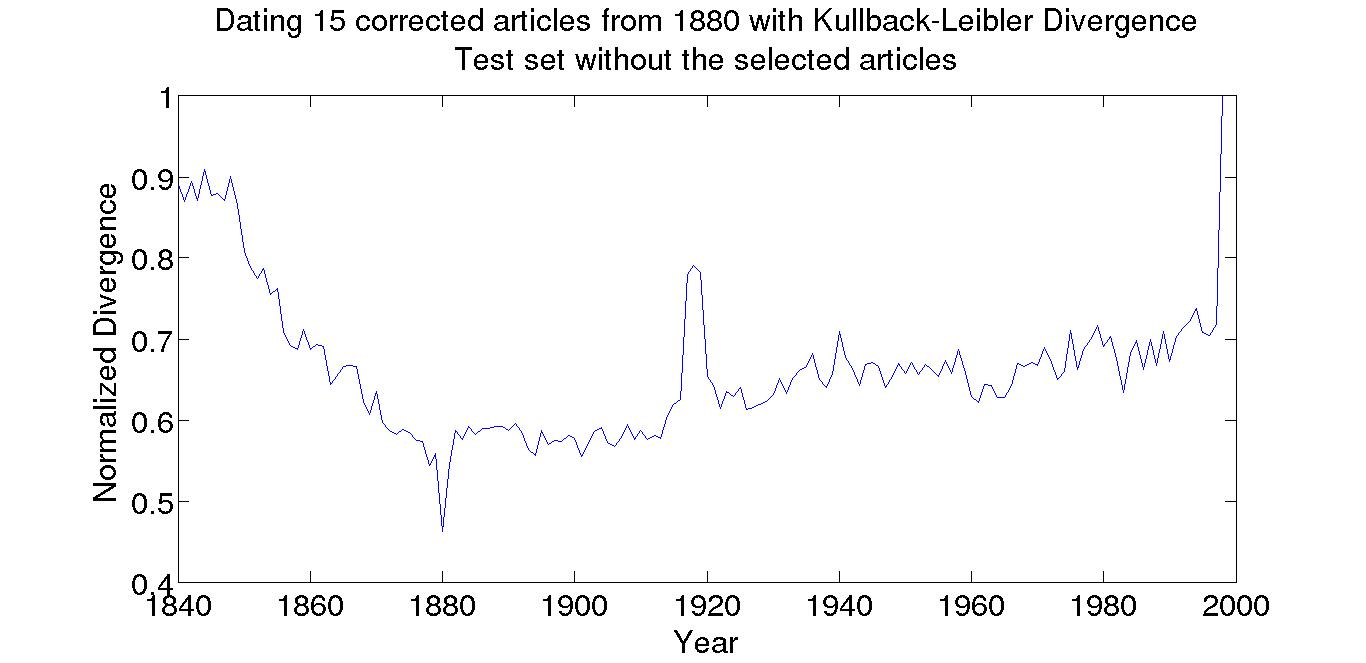
\includegraphics[scale=0.15]{Pictures/date_articles/kullback_leibler/15articles_1880_KL_years_simulate_articles_corrected_without_articles.jpg}
        \caption{KL for 15 articles with OCR correction for year 1880}
        \label{ArticleKL-C1880}
    \end{minipage}\hfill
    \begin{minipage}[b]{0.5\linewidth}
        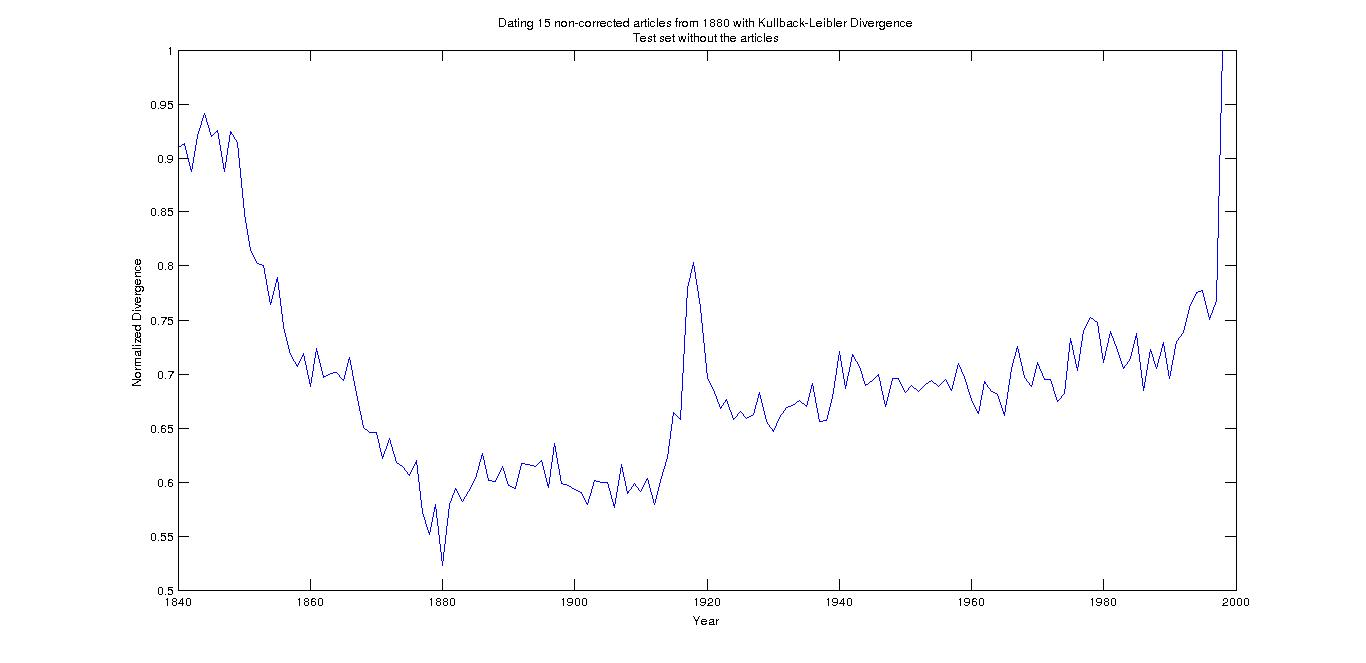
\includegraphics[scale=0.15]{Pictures/date_articles/kullback_leibler/15articles_1880_KL_years_simulate_articles_without_correction_without_articles.jpg}
        \caption{KL for 15 articles without OCR correction for year 1880}
        \label{ArticleKL-N1880}
    \end{minipage}\hfill
\end{figure}

\begin{figure}[h!]
    \begin{minipage}[b]{0.48\linewidth}
        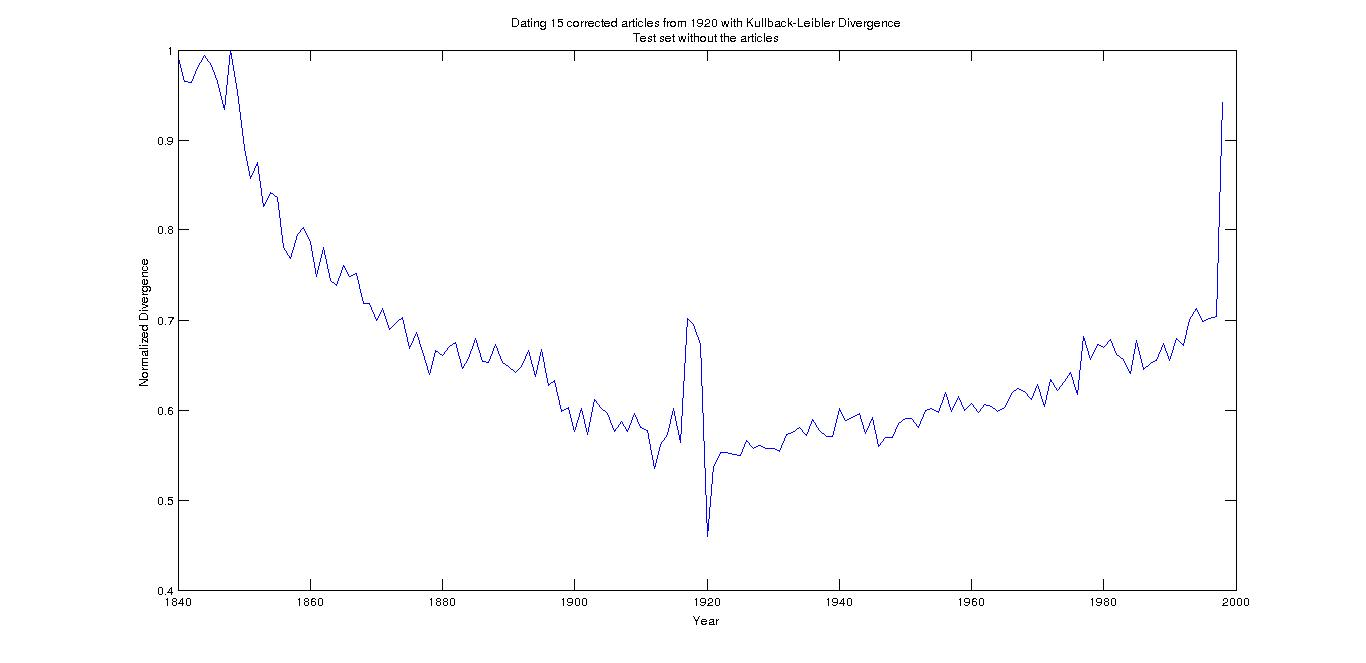
\includegraphics[scale=0.15]{Pictures/date_articles/kullback_leibler/15articles_1920_KL_years_simulate_articles_corrected_without_articles.jpg}
        \caption{KL for 15 articles with OCR correction for year 1920}
        \label{ArticleKL-C1920}
    \end{minipage}\hfill
    \begin{minipage}[b]{0.5\linewidth}
        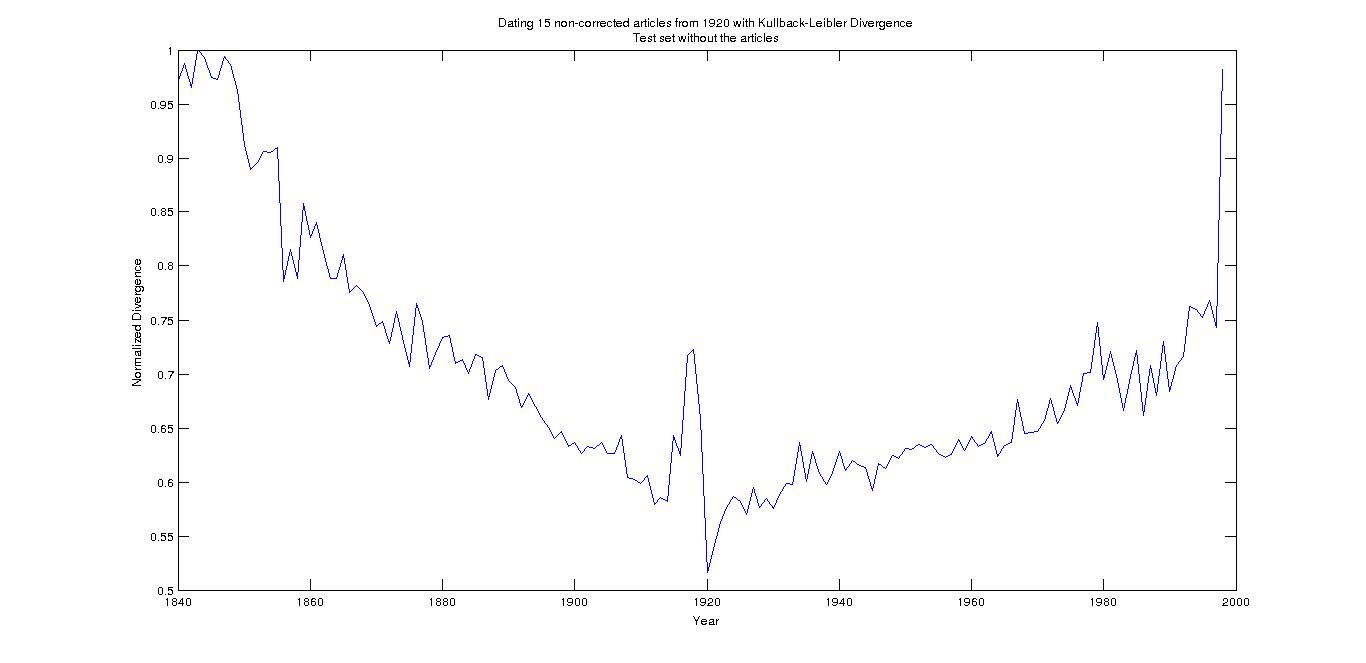
\includegraphics[scale=0.15]{Pictures/date_articles/kullback_leibler/15articles_1920_KL_years_simulate_articles_without_correction_without_articles.jpg}
        \caption{KL for 15 articles without OCR correction for year 1920}
        \label{ArticleKL-N1920}
    \end{minipage}\hfill
\end{figure}

\begin{figure}[h!]
    \begin{minipage}[b]{0.48\linewidth}
        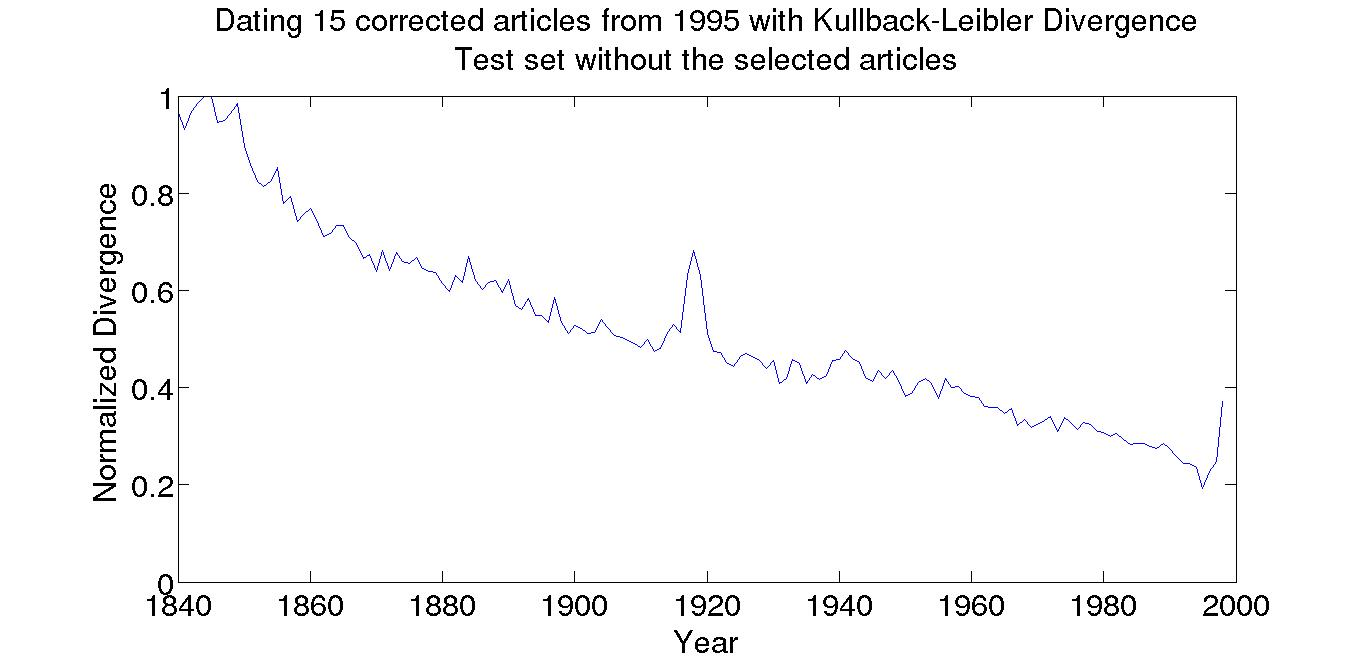
\includegraphics[scale=0.15]{Pictures/date_articles/kullback_leibler/15articles_1995_KL_years_simulate_articles_corrected_without_articles.jpg}
        \caption{KL for 15 articles with OCR correction for year 1995}
        \label{ArticleKL-C1995}
    \end{minipage}\hfill
    \begin{minipage}[b]{0.5\linewidth}
        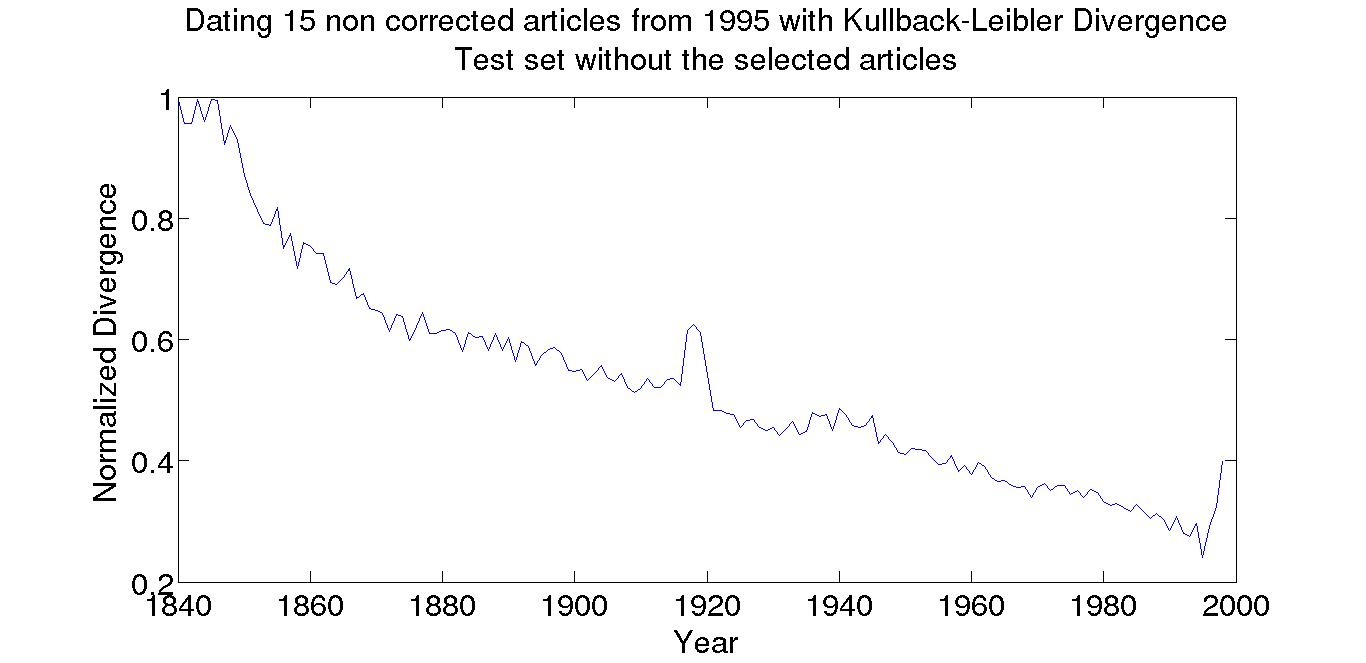
\includegraphics[scale=0.15]{Pictures/date_articles/kullback_leibler/15articles_1995_KL_years_simulate_articles_without_correction_without_articles.jpg}
        \caption{KL for 15 articles without OCR correction for year 1995}
        \label{ArticleKL-N1995}
    \end{minipage}\hfill
\end{figure}

We took only the direction where the year approximate the articles because it has no sense to do the inverse. Indeed, to approximate a year that contains thousands of words with a subset of articles that contains a few hundred words will lead to a dating that will very often predict the years with less words (in the 19$th$ century).

We can observe again in these figures that the OCR correction does not help so much for dating. But, we can observe that the \emph{Kullback-Leibler} Divergence is really good to date the articles. Our explanation for these excellent results is that when we remove some articles from a year, the probability that the words are present in this year is higher than in other years. So, even if we remove the articles from the year, it stays hardly attached to the article and when the year approximate the articles, it has a really good matching.

\subsubsection{Out of Place}
\subsubsection{Punctuation and sentences length}
As the statistics on punctuation and sentences tend to change between years (especially for the sentences lengths and number of commas), we tried to implement a metric with those statistics. \\

Those statistics are extracted for each year and combined in a single entry by year. For the metric, we take a sample of articles from one year, we merge them, as it was one big article, we compute the statistics on this article and we use a simple euclidean distance to compute the distance with each year. The result for a sample of 15 random articles from 1925 is observable in figure \ref{punct_metric_1925}.

\begin{figure}[H]
	\centering
    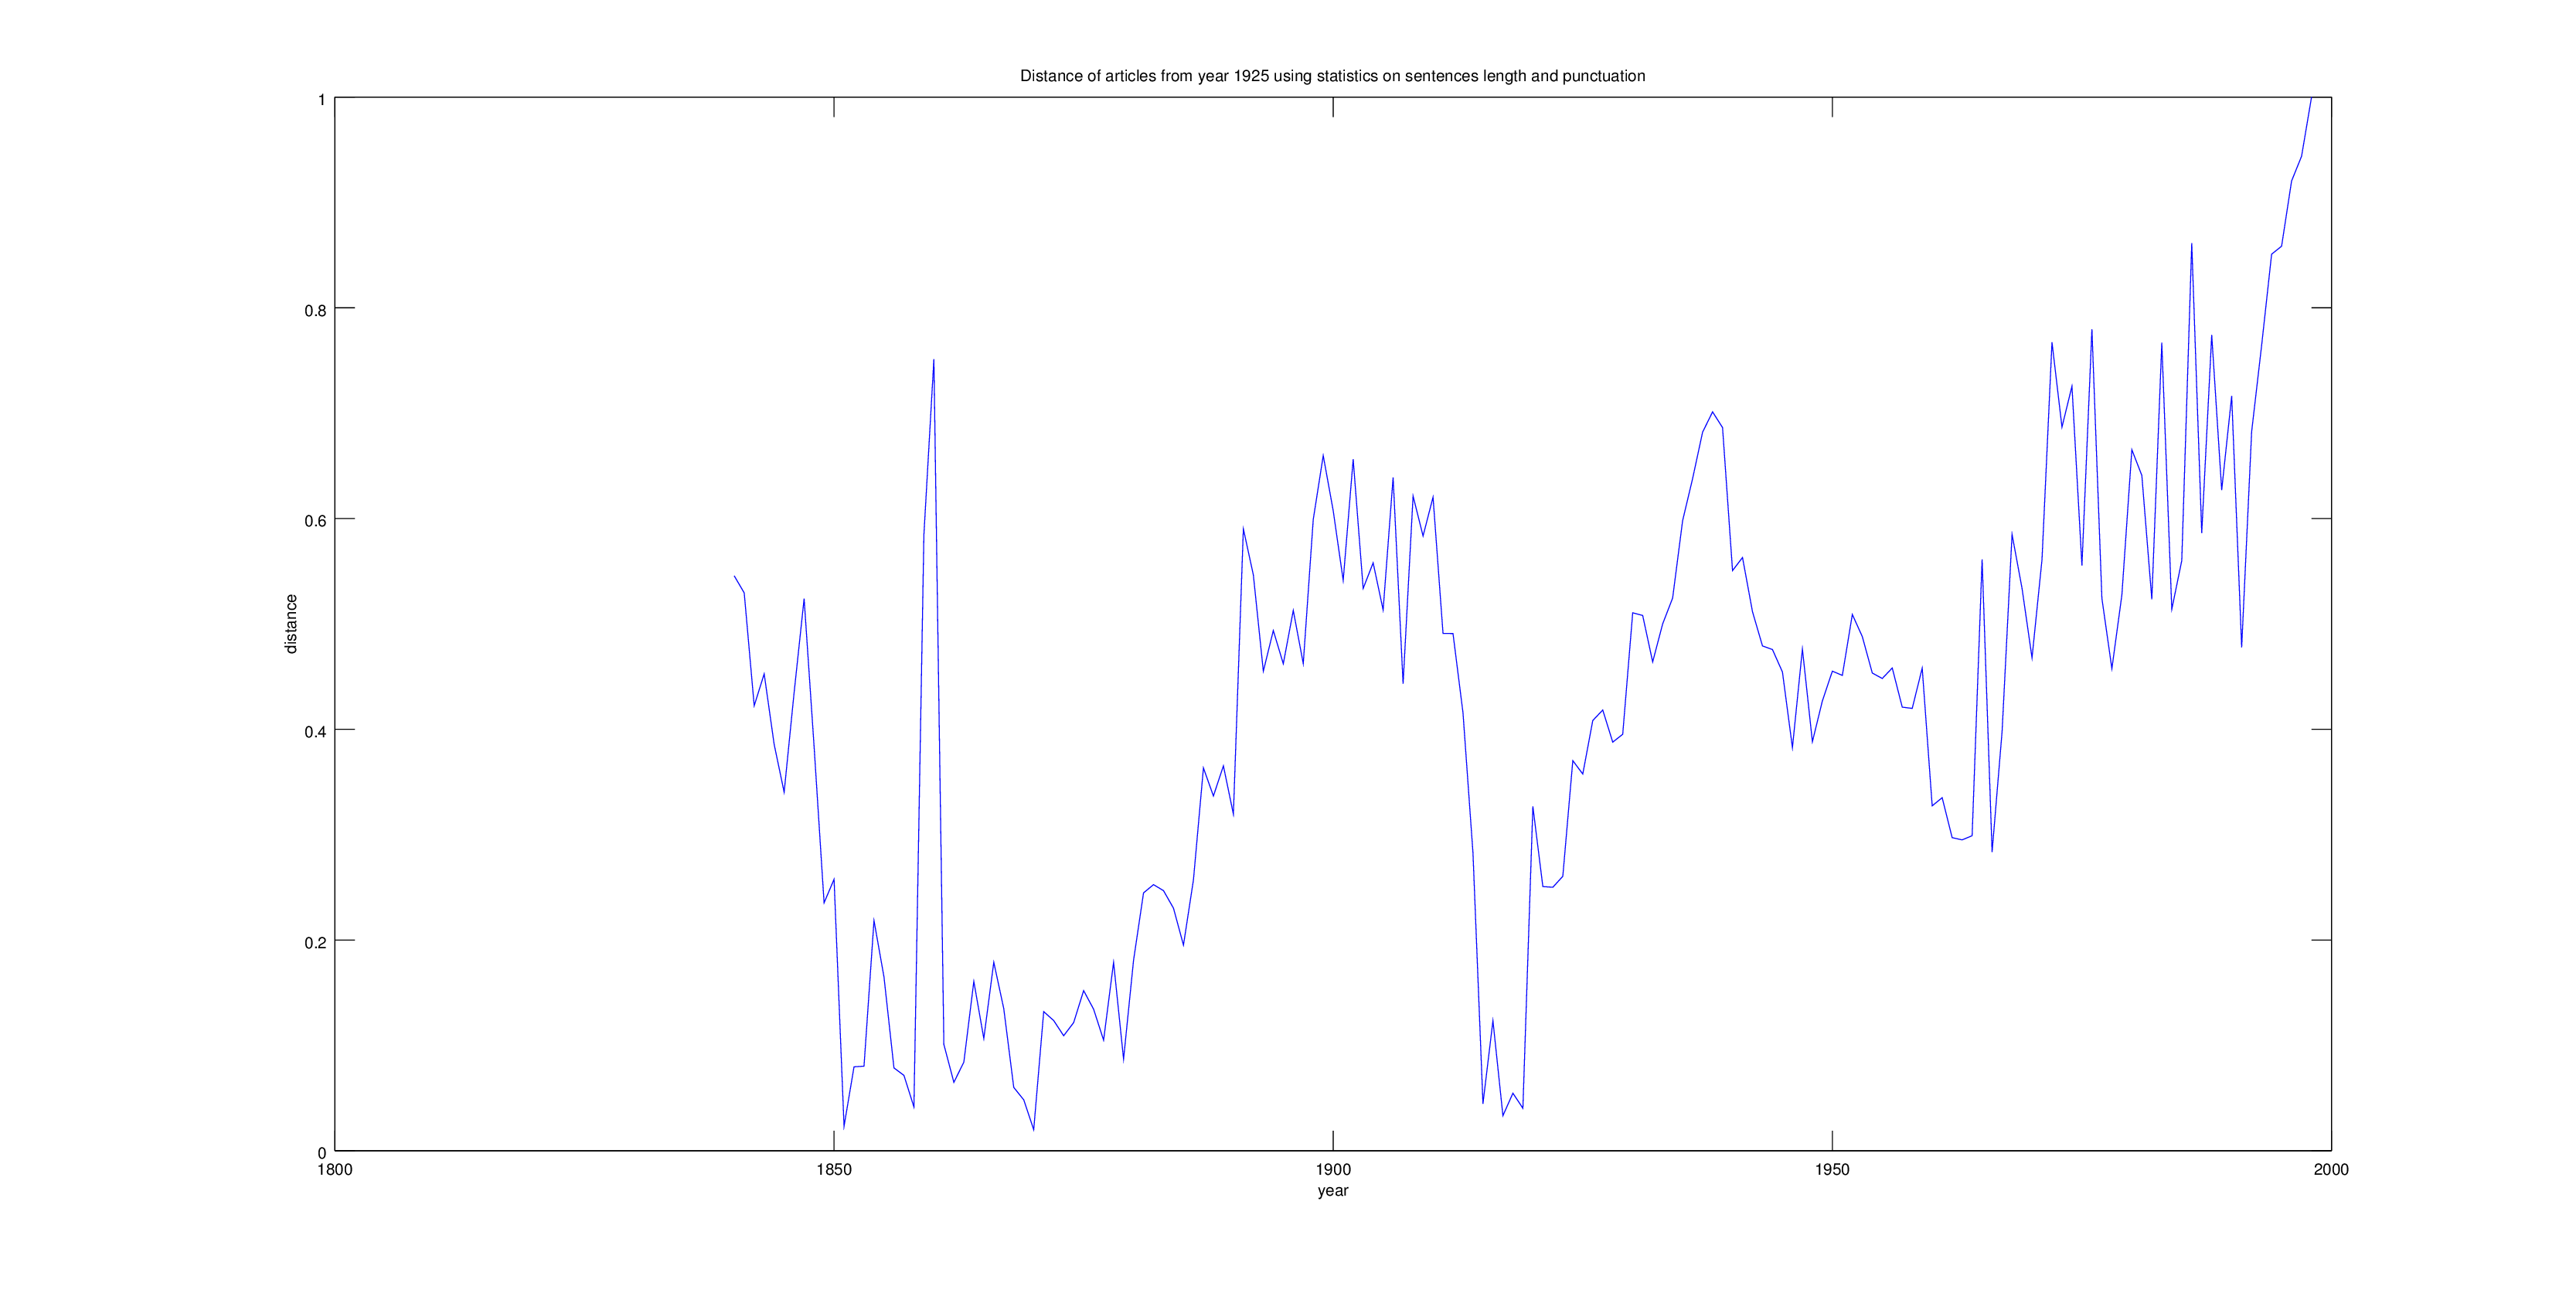
\includegraphics[scale=0.5]{Pictures/date_articles/punctuation/graph.png}
    \caption{Distance between a sample of 15 random articles from 1925 and each year}
    \label{punct_metric_1925}\hfill
\end{figure}

As we can see, it does not work that well, but with more time, we could have used machine learning methods instead of a simple euclidean distance, we think it could be useful to combine the result obtained them with other distances to enhance the classification.

\subsection{Cross Validation}
To have stronger values when we date articles, we wrote a script that runs several times each metrics for a different subsets of article of the same year. The idea here is to have an average on the error of each metric to be able to compare them together. We obtained the following results for random years.\\

\textbf{Mean error for different metrics for 15 articles in year 1843 with 15 iterations}\\
\begin{tabular}{p{3cm} p{5cm}}
Distance1 :& 0\\
Cosine :& 10.73333333333333333333\\
Cosine-TFIDF :& .40000000000000000000\\
Chi-Square :& 112.40000000000000000000\\
Kullback-Leibler :& 11.33333333333333333333\\
OutOfPlace :& 3.00000000000000000000\\
Punctuation :& 33.13333333333333333333\\
\end{tabular}\\
 
\textbf{Mean error for different metrics for 15 articles in year 1854 with 15 iterations}\\
\begin{tabular}{p{3cm} p{5cm}}
    Distance1 :& 8.00000000000000000000\\
    Cosine :& 9.86666666666666666666\\
    Cosine-TFIDF :& 0\\
    Chi-Square :& 111.86666666666666666666\\
    Kullback-Leibler :& 0\\
    OutOfPlace :& 8.00000000000000000000\\
    Punctuation :& 15.80000000000000000000\\
\end{tabular}\\
 
\textbf{Mean error for different metrics for 15 articles in year 1888 with 15 iterations}\\
\begin{tabular}{p{3cm} p{5cm}}
    Distance1 :& 42.00000000000000000000\\
    Cosine :& 15.13333333333333333333\\
    Cosine-TFIDF :& 0\\
    Chi-Square :& 62.40000000000000000000\\
    Kullback-Leibler :& .26666666666666666666\\
    OutOfPlace :& 42.00000000000000000000\\
    Punctuation :& 32.80000000000000000000\\
\end{tabular}\\
 
\textbf{Mean error for different metrics for 15 articles in year 1905 with 15 iterations}\\
\begin{tabular}{p{3cm} p{5cm}}
    Distance1 :& 65.80000000000000000000\\
    Cosine :& 17.13333333333333333333\\
    Cosine-TFIDF :& .06666666666666666666\\
    Chi-Square :& 48.40000000000000000000\\
    Kullback-Leibler :& 3.06666666666666666666\\
    OutOfPlace :& 59.00000000000000000000\\
    Punctuation :& 21.06666666666666666666\\
\end{tabular}\\
 
\textbf{Mean error for different metrics for 15 articles in year 1918 with 15 iterations}\\
\begin{tabular}{p{3cm} p{5cm}}
    Distance1 :& 78.93333333333333333333\\
    Cosine :& 4.73333333333333333333\\
    Cosine-TFIDF :& 0\\
    Chi-Square :& 36.33333333333333333333\\
    Kullback-Leibler :& 2.66666666666666666666\\
    OutOfPlace :& 72.00000000000000000000\\
    Punctuation :& 30.86666666666666666666\\
\end{tabular}\\
 
\textbf{Mean error for different metrics for 15 articles in year 1934 with 15 iterations}\\
\begin{tabular}{p{3cm} p{5cm}}
    Distance1 :& 65.60000000000000000000\\
    Cosine :& 17.46666666666666666666\\
    Cosine-TFIDF :& .80000000000000000000\\
    Chi-Square :& 128.93333333333333333333\\
    Kullback-Leibler :& .33333333333333333333\\
    OutOfPlace :& 88.00000000000000000000\\
    Punctuation :& 37.66666666666666666666\\
\end{tabular}\\
 
\textbf{Mean error for different metrics for 15 articles in year 1954 with 15 iterations}\\
\begin{tabular}{p{3cm} p{5cm}}
    Distance1 :& 44.00000000000000000000\\
    Cosine :& 24.60000000000000000000\\
    Cosine-TFIDF :& 0\\
    Chi-Square :& 0\\
    Kullback-Leibler :& .66666666666666666666\\
    OutOfPlace :& 108.00000000000000000000\\
    Punctuation :& 48.06666666666666666666\\
\end{tabular}\\
 
\textbf{Mean error for different metrics for 15 articles in year 1984 with 15 iterations}\\
\begin{tabular}{p{3cm} p{5cm}}
    Distance1 :& 14.00000000000000000000\\
    Cosine :& 7.20000000000000000000\\
    Cosine-TFIDF :& 1.66666666666666666666\\
    Chi-Square :& 3.73333333333333333333\\
    Kullback-Leibler :& 0\\
    OutOfPlace :& 138.00000000000000000000\\
    Punctuation :& 81.80000000000000000000\\
\end{tabular}\\

We observe that two metrics are in general better than the others. These two metrics are the \emph{Kullback-Leibler} Divergence and the Cosine with TF-IDF. Indeed, as explained in section \ref{metrics}, these two metrics are good and we know why. The other metrics are not so bad, even the basic distance which has surprisingly an error of 0 when dating articles from 1843. We think this distance was just lucky with the subset of articles. TOOOOOOOOOOOOOOOOOOOOOOOOODDDDDDDDDDDDDDDOOOOOOOOOOOOOOOOOOOOOOOOOOOO Indeed, we have run the dating of articles with the same options but with different subsets of articles and we can observe that the basic distance is not anymore equal to 0. For the other metrics, we can observe that they vary depending on the year or certainly on the subset of articles.\\

To judge which metric is the best one, we can simply compute the mean error over all our samples. As it takes a lot of time to compute 15 times each metrics, we can't compute it for each year. Here is the overall mean over all the years we tested :\\

\textbf{Mean error for different metrics for 15 articles in the years selected above with 15 iterations per year}\\
\begin{tabular}{p{3cm} p{5cm}}
    Distance1 :& 39.7875\\
    Cosine :& 13.35875\\
    Cosine-TFIDF :& 0.36675\\
    Chi-Square :& 63.008625\\
    Kullback-Leibler :& 2.292\\
    OutOfPlace :& 64.75\\
    Punctuation :& 37.65025\\
\end{tabular}\\

We can observe that, as expected, Cosine with TF-IDF distance and \emph{Kullback-Leibler} Divergence are the best ones.\\

Finally, we made some tests to compare, for a given year, if the number of selected articles to date changes a lot the results of the metrics. And....

\section{Topics}\label{topics}

We wanted to see how is the evolution of the language inside a specific topic of the corpus (e.g. swiss politics, sport, art,...).	
Our idea was that a topic clustering would help us capture the linguistic drift more precisely when comparing two articles that talk about the same subject.
This new approach would give us different results.\\
For topic clustering, we chose to use \emph{Latent Dirichlet Allocation} (LDA) implemented in spark since spark 1.3.0. 
The algorithms take as input a matrix of article and 1-gram occurrences and cluster the articles into a specified number \textit{n} of topics. We could also set te parameters for topic distribution over terms $\beta$ and articles distribution over topics $\alpha$. Empirical results led us to set the $\beta$ to 17, a relatively high value because articles contain lot of stop words that could have too much weight for lower values. In the same way, we set $\alpha$ to 1.1, the minimum value, as articles in a newspaper would rather belong to a single topic. For a number of topics equal to \textit{n} equal to 20.\\

\subsection{Metrics with Topics}
In order to measure the linguistic drift over the topics we constrain ourselves with two metrics: Kullback-Leibler and Cosine. Simply because these two gave us the better results beforehand. 
\subsubsection{Cosine Similarity}

With the cosine based distance, it seems that the fact that the articles are separated into topics makes a better contrast appear between the years. Indeed, because the years are represented by vectors containing the frequencies of the words, and that the dimension of those vectors is reduced by the number of words that are specific for other topics, then if the angle is big, it is due to the language itself and note more on the fact that it can be on opposed subjects.

\begin{figure}[H]
    \begin{minipage}[b]{0.48\linewidth}
        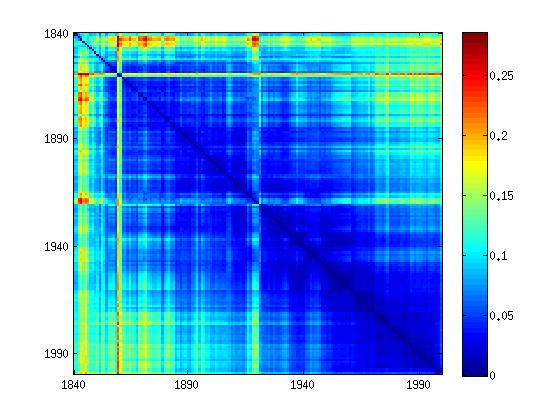
\includegraphics[scale=0.3]{Pictures/topics/cos/topic1.jpg}
        \caption{cosine distance on topic 1: history}
        \label{cos_topic1}
    \end{minipage}\hfill
    \begin{minipage}[b]{0.5\linewidth}
        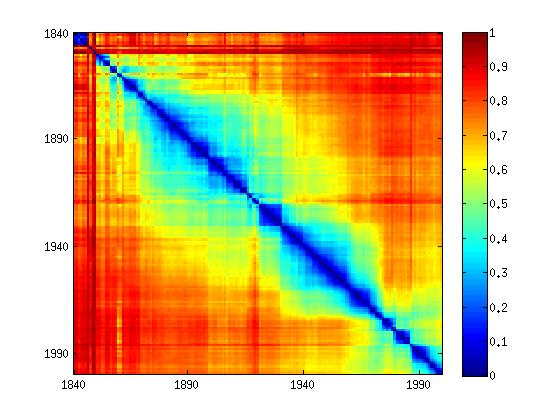
\includegraphics[scale=0.3]{Pictures/topics/cos/topic3.jpg}
        \caption{cosine distance on topic 3: general}
        \label{cos_topic3}
    \end{minipage}\hfill
\end{figure}

There is some topics where we cannot distinguish any drift where an example is shown in figure \ref{cos_topic1}. The concerned topic is about history and religion, so it seems legit that it doesn't change over years and the language drift is hard to enhance for that kind of subject. On the contrary, there is some topics where a drift over years is well marked such as in figure \ref{cos_topic3}. For those cases, the fact that the articles are separated in topics gives an improvement for the cosine metric.

\begin{figure}[H]
    \begin{minipage}[b]{0.48\linewidth}
        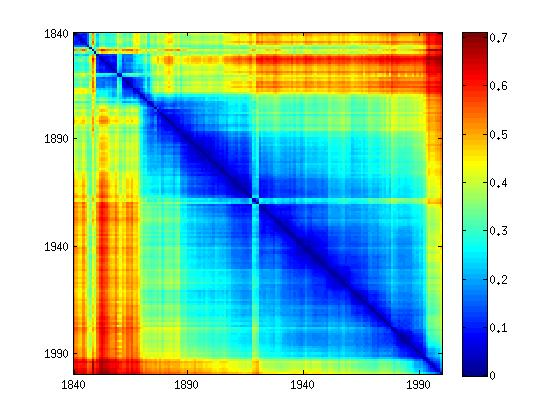
\includegraphics[scale=0.3]{Pictures/topics/cos/topic7.jpg}
        \caption{cosine distance on topic 7: Swiss politics}
        \label{cos_topic7}
    \end{minipage}\hfill
    \begin{minipage}[b]{0.5\linewidth}
        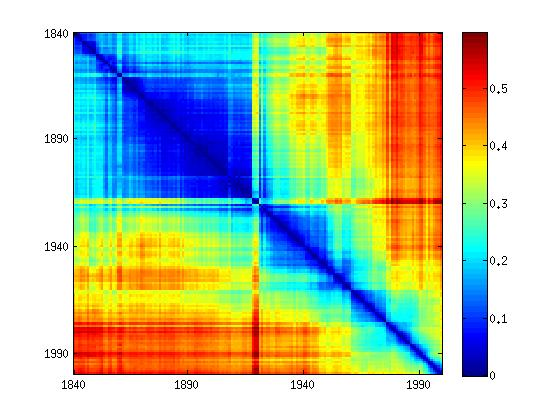
\includegraphics[scale=0.3]{Pictures/topics/cos/topic9.jpg}
        \caption{cosine distance on topic 9: theatre and music}
        \label{cos_topic9}
    \end{minipage}\hfill
\end{figure}

We have also interesting topics such as Swiss politics or music in figures \ref{cos_topic7} and \ref{cos_topic9} where a drift is also enhanced compared to the distance on the whole corpus but the changes are not proportional along the time.
\subsubsection{Kullback-Leibler Divergence}

The computations between years for a given topic give some waited results. Indeed, as you can see in figures \ref{KL-topic7} and \ref{KL-topic1}, the divergence between years is really small. Especially for the topic 'swiss politic' because the words that are present in this topic ('confédération', 'suisse', 'fédéral', ...) are words that are used every year. Thus, when a year approximate another one, this is almost perfect. There is just an exception for the years 1840 to 1848 that have difficulties to approximate other years. It is easily explicable because the swiss federal state was created in 1848 so the vocabulary for the 'swiss politic' was not exactly the same between 1840 and 1848.

For a more general topic like 'culture', we can observe the same behaviour that have the \emph{Kullback-Leibler} Divergence without using the topics (see section \ref{metrics}). Indeed, the vocabulary for 'culture' should increase over years, so years of the 19$th$ century have more difficulties to approximate the years of the 20$th$ century and it is not the case in the other direction.

We can also note that use \emph{Kullback-Leibler} divergence to date articles is not a good idea, due to the general plots with the topics.


\begin{figure}[h!]
    \begin{minipage}[b]{0.48\linewidth}
        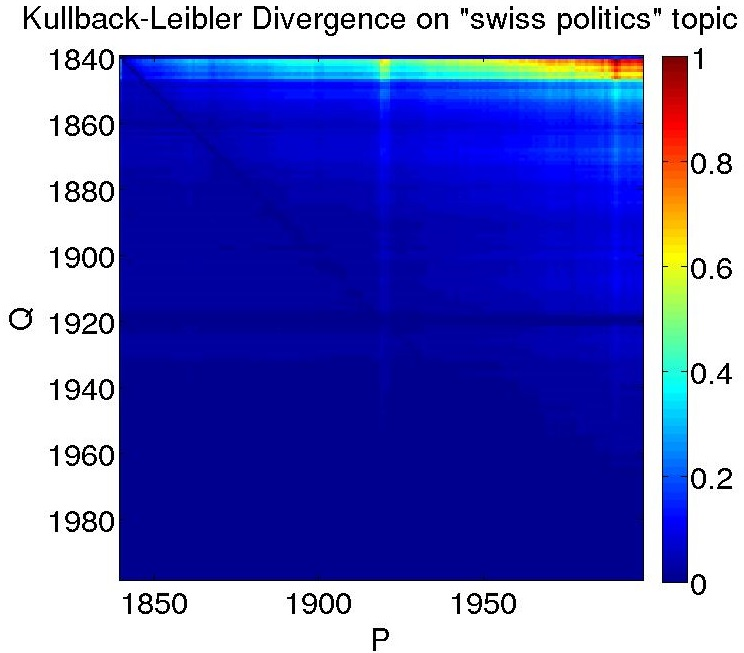
\includegraphics[scale=0.15]{Pictures/topics/kullback-leibler/KL_topic7.jpg}
        \caption{KL for the topic 'swiss politic'}
        \label{KL-topic7}
    \end{minipage}\hfill
    \begin{minipage}[b]{0.5\linewidth}
        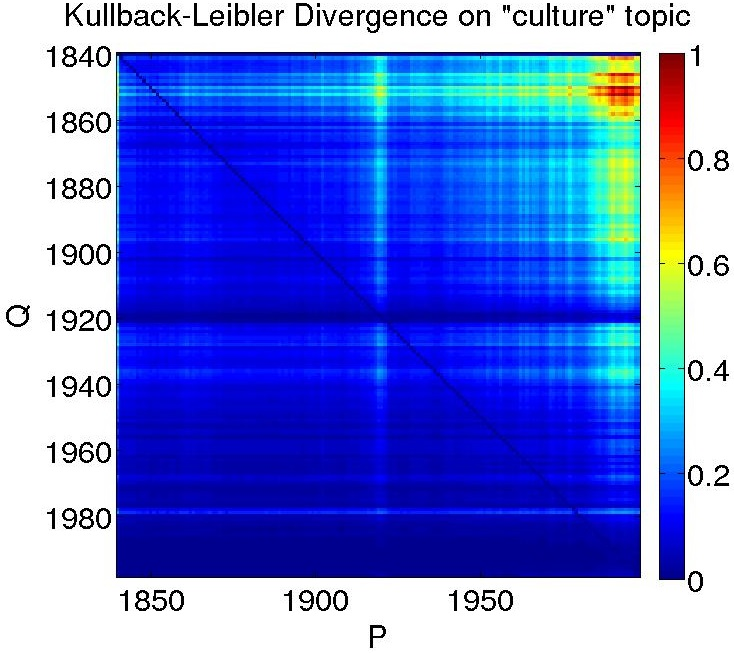
\includegraphics[scale=0.15]{Pictures/topics/kullback-leibler/KL_topic1.jpg}
        \caption{KL for the topic 'culture'}
        \label{KL-topic1}
    \end{minipage}\hfill
\end{figure}

Finally, for all the 15 topics that were extracted from the corpus, the divergence between years are well represented by the 2 examples in figures \ref{KL-topic7} and \ref{KL-topic1}. For topics that have vocabulary that not really changes over time, the divergence will be of the same kind as for the 'swiss politic' topic and and for the other it will be like the 'culture' topic.

\section{Conclusion}\label{conclusion}
To conclude this report, we can say that there exists a linguistic drift in our newspaper's corpus. Indeed, a straightforward statement is that we use more vocabulary to express the same ideas and we do shorter sentences. We also observed that the gain on words through is more important than words disappearances.

About the OCR correction, we saw that for some metrics the correction doesn't have any influence but for other ones (in particular for cosine distance), it helps to improve the observation of the linguistic drift. Then, with the TF-IDF values, it is again the cosine metric that benefits from the importance of uncommon words. For the other metrics, it is less useful.

Then, when we tried to date articles, we obtained some really good results using the \emph{Kullback-Leibler} Divergence and the cosine distance with TF-IDF. Indeed, with those two metrics, we were able to date a subset of articles with less than 10 years error in general what could be considered as an indicator of the goodness of these metrics. With the other metrics, the error is a bit bigger, but they can have sometimes some good results due to some specific reasons (like the number of words in the year).

Finally, with the topics, we found some interesting ones for which we were able to found some properties using the \emph{Kullback-Leibler} Divergence and the cosine distance. Indeed, with the KL divergence, we saw that years in general are not divergent to each other and with cosine we saw that years that are close have a small distance between them.



\end{document}